\PassOptionsToPackage{unicode=true}{hyperref} % options for packages loaded elsewhere
\PassOptionsToPackage{hyphens}{url}
%
\documentclass[
]{book}
\usepackage{lmodern}
\usepackage{amssymb,amsmath}
\usepackage{ifxetex,ifluatex}
\ifnum 0\ifxetex 1\fi\ifluatex 1\fi=0 % if pdftex
  \usepackage[T1]{fontenc}
  \usepackage[utf8]{inputenc}
  \usepackage{textcomp} % provides euro and other symbols
\else % if luatex or xelatex
  \usepackage{unicode-math}
  \defaultfontfeatures{Scale=MatchLowercase}
  \defaultfontfeatures[\rmfamily]{Ligatures=TeX,Scale=1}
\fi
% use upquote if available, for straight quotes in verbatim environments
\IfFileExists{upquote.sty}{\usepackage{upquote}}{}
\IfFileExists{microtype.sty}{% use microtype if available
  \usepackage[]{microtype}
  \UseMicrotypeSet[protrusion]{basicmath} % disable protrusion for tt fonts
}{}
\makeatletter
\@ifundefined{KOMAClassName}{% if non-KOMA class
  \IfFileExists{parskip.sty}{%
    \usepackage{parskip}
  }{% else
    \setlength{\parindent}{0pt}
    \setlength{\parskip}{6pt plus 2pt minus 1pt}}
}{% if KOMA class
  \KOMAoptions{parskip=half}}
\makeatother
\usepackage{xcolor}
\IfFileExists{xurl.sty}{\usepackage{xurl}}{} % add URL line breaks if available
\IfFileExists{bookmark.sty}{\usepackage{bookmark}}{\usepackage{hyperref}}
\hypersetup{
  pdftitle={Machine Learning},
  pdfauthor={Elton Massahiro Saito Loures},
  pdfborder={0 0 0},
  breaklinks=true}
\urlstyle{same}  % don't use monospace font for urls
\usepackage{color}
\usepackage{fancyvrb}
\newcommand{\VerbBar}{|}
\newcommand{\VERB}{\Verb[commandchars=\\\{\}]}
\DefineVerbatimEnvironment{Highlighting}{Verbatim}{commandchars=\\\{\}}
% Add ',fontsize=\small' for more characters per line
\usepackage{framed}
\definecolor{shadecolor}{RGB}{248,248,248}
\newenvironment{Shaded}{\begin{snugshade}}{\end{snugshade}}
\newcommand{\AlertTok}[1]{\textcolor[rgb]{0.94,0.16,0.16}{#1}}
\newcommand{\AnnotationTok}[1]{\textcolor[rgb]{0.56,0.35,0.01}{\textbf{\textit{#1}}}}
\newcommand{\AttributeTok}[1]{\textcolor[rgb]{0.77,0.63,0.00}{#1}}
\newcommand{\BaseNTok}[1]{\textcolor[rgb]{0.00,0.00,0.81}{#1}}
\newcommand{\BuiltInTok}[1]{#1}
\newcommand{\CharTok}[1]{\textcolor[rgb]{0.31,0.60,0.02}{#1}}
\newcommand{\CommentTok}[1]{\textcolor[rgb]{0.56,0.35,0.01}{\textit{#1}}}
\newcommand{\CommentVarTok}[1]{\textcolor[rgb]{0.56,0.35,0.01}{\textbf{\textit{#1}}}}
\newcommand{\ConstantTok}[1]{\textcolor[rgb]{0.00,0.00,0.00}{#1}}
\newcommand{\ControlFlowTok}[1]{\textcolor[rgb]{0.13,0.29,0.53}{\textbf{#1}}}
\newcommand{\DataTypeTok}[1]{\textcolor[rgb]{0.13,0.29,0.53}{#1}}
\newcommand{\DecValTok}[1]{\textcolor[rgb]{0.00,0.00,0.81}{#1}}
\newcommand{\DocumentationTok}[1]{\textcolor[rgb]{0.56,0.35,0.01}{\textbf{\textit{#1}}}}
\newcommand{\ErrorTok}[1]{\textcolor[rgb]{0.64,0.00,0.00}{\textbf{#1}}}
\newcommand{\ExtensionTok}[1]{#1}
\newcommand{\FloatTok}[1]{\textcolor[rgb]{0.00,0.00,0.81}{#1}}
\newcommand{\FunctionTok}[1]{\textcolor[rgb]{0.00,0.00,0.00}{#1}}
\newcommand{\ImportTok}[1]{#1}
\newcommand{\InformationTok}[1]{\textcolor[rgb]{0.56,0.35,0.01}{\textbf{\textit{#1}}}}
\newcommand{\KeywordTok}[1]{\textcolor[rgb]{0.13,0.29,0.53}{\textbf{#1}}}
\newcommand{\NormalTok}[1]{#1}
\newcommand{\OperatorTok}[1]{\textcolor[rgb]{0.81,0.36,0.00}{\textbf{#1}}}
\newcommand{\OtherTok}[1]{\textcolor[rgb]{0.56,0.35,0.01}{#1}}
\newcommand{\PreprocessorTok}[1]{\textcolor[rgb]{0.56,0.35,0.01}{\textit{#1}}}
\newcommand{\RegionMarkerTok}[1]{#1}
\newcommand{\SpecialCharTok}[1]{\textcolor[rgb]{0.00,0.00,0.00}{#1}}
\newcommand{\SpecialStringTok}[1]{\textcolor[rgb]{0.31,0.60,0.02}{#1}}
\newcommand{\StringTok}[1]{\textcolor[rgb]{0.31,0.60,0.02}{#1}}
\newcommand{\VariableTok}[1]{\textcolor[rgb]{0.00,0.00,0.00}{#1}}
\newcommand{\VerbatimStringTok}[1]{\textcolor[rgb]{0.31,0.60,0.02}{#1}}
\newcommand{\WarningTok}[1]{\textcolor[rgb]{0.56,0.35,0.01}{\textbf{\textit{#1}}}}
\usepackage{longtable,booktabs}
% Allow footnotes in longtable head/foot
\IfFileExists{footnotehyper.sty}{\usepackage{footnotehyper}}{\usepackage{footnote}}
\makesavenoteenv{longtable}
\usepackage{graphicx,grffile}
\makeatletter
\def\maxwidth{\ifdim\Gin@nat@width>\linewidth\linewidth\else\Gin@nat@width\fi}
\def\maxheight{\ifdim\Gin@nat@height>\textheight\textheight\else\Gin@nat@height\fi}
\makeatother
% Scale images if necessary, so that they will not overflow the page
% margins by default, and it is still possible to overwrite the defaults
% using explicit options in \includegraphics[width, height, ...]{}
\setkeys{Gin}{width=\maxwidth,height=\maxheight,keepaspectratio}
\setlength{\emergencystretch}{3em}  % prevent overfull lines
\providecommand{\tightlist}{%
  \setlength{\itemsep}{0pt}\setlength{\parskip}{0pt}}
\setcounter{secnumdepth}{5}
% Redefines (sub)paragraphs to behave more like sections
\ifx\paragraph\undefined\else
  \let\oldparagraph\paragraph
  \renewcommand{\paragraph}[1]{\oldparagraph{#1}\mbox{}}
\fi
\ifx\subparagraph\undefined\else
  \let\oldsubparagraph\subparagraph
  \renewcommand{\subparagraph}[1]{\oldsubparagraph{#1}\mbox{}}
\fi

% set default figure placement to htbp
\makeatletter
\def\fps@figure{htbp}
\makeatother

\usepackage{booktabs}
\usepackage[utf8]{inputenc}
\usepackage{amsthm}
\makeatletter
\def\thm@space@setup{%
  \thm@preskip=8pt plus 2pt minus 4pt
  \thm@postskip=\thm@preskip
}
\makeatother
\usepackage[]{natbib}
\bibliographystyle{apalike}

\title{Machine Learning}
\author{Elton Massahiro Saito Loures}
\date{2020-12-02}

\begin{document}
\maketitle

{
\setcounter{tocdepth}{1}
\tableofcontents
}
\hypertarget{prefuxe1cio}{%
\chapter*{Prefácio}\label{prefuxe1cio}}
\addcontentsline{toc}{chapter}{Prefácio}

\hypertarget{por-que-ler-esse-livro}{%
\section{Por que ler esse livro?}\label{por-que-ler-esse-livro}}

\hypertarget{estrutura}{%
\section{Estrutura}\label{estrutura}}

\hypertarget{informauxe7uxf5es-a-respeito-do-conteuxfado}{%
\section{Informações a respeito do conteúdo}\label{informauxe7uxf5es-a-respeito-do-conteuxfado}}

\hypertarget{agradecimentos}{%
\section{Agradecimentos}\label{agradecimentos}}

\begin{Shaded}
\begin{Highlighting}[]
\KeywordTok{install.packages}\NormalTok{(}\StringTok{"bookdown"}\NormalTok{)}
\CommentTok{# or the development version}
\CommentTok{# devtools::install_github("rstudio/bookdown")}
\end{Highlighting}
\end{Shaded}

Remember each Rmd file contains one and only one chapter, and a chapter is defined by the first-level heading \texttt{\#}.

To compile this example to PDF, you need XeLaTeX. You are recommended to install TinyTeX (which includes XeLaTeX): \url{https://yihui.name/tinytex/}.

\hypertarget{intro}{%
\chapter{Introdução}\label{intro}}

Caro leitor, se você veio até esse livro é bem provável que passou e/ou ainda passa pelas mesmas dificuldades que todo estudante interessado nessa área.

Ao elevado número de pesquisas que fiz para aprender o que era a Inteligência Artificial, o que era o \emph{Machine Learning} (Aprendizado de Máquina) e todos os outros temas similares, é nítido que ainda não está totalmente definido o conceito de cada um. É um ramo novo na área acadêmica, na indústria e em todo o mercado, com diversos temas, diversos modelos matemáticos, diversos modelos computacionais, diversos \emph{softwares}, diversas aplicações e em diversas áreas. Diversos ``diversos''\ldots{} E o mais assustador é que esse campo une todos esses ``diversos'', tornando o universo \textbf{caótico} ainda maior. Quando destaco o termo ``caótico'', refiro exatamente pela ironia deste mote, todo esse universo confuso é aplicado em nosso cotidiano para organizar, analisar, diagnosticar e facilitar as coisas.

Poucos instruem como devemos enxergar todo esse cosmos que ao longo da história está passando por diversas construções para estruturar seu conceito. Com uma tentativa de trazer isso com base em artigos, livros, vídeos, podcasts e cursos, disponho este simples livro com o propósito de organizar a imagem que você, leitor, tem de Aprendizado de Máquina e entender os principais modelos utilizados tanto no meio acadêmico, quanto no mercado de trabalho.

\hypertarget{dicas-de-estudo}{%
\section{Dicas de estudo}\label{dicas-de-estudo}}

Não cabe a mim dizer como estudar, mas o que posso lhe aconselhar como principal ponto é a \textbf{paciência}. Temas como esse podem abranger qualquer campo, desde a filosofia até a área da saúde e portanto, do mesmo modo que se aplica a qualquer conteúdo, o mais importante é a base. Leia, releia, pesquise, veja vídeos, ouça um podcast, converse e discuta com colegas e professores a respeito. Não se cobre de que precisa aprender o mais rápido possível, mas preze a qualidade do estudo.

Com intuito de explicar sobre Aprendizado de Máquina. Na seção \textbf{AQUI VOU COLOCAR A REFERENCIA DA SESSAO}, para faciliar o leitor dependendo de sua demanda de conteúdo, busquei separar em subseções a lógica computacional e a matemática. Tornando mais prático para o público que não tem interesse no modelo matemático e que busca o conhecimento de determinado assunto quanto ao público que demanda esse conteúdo.

\hypertarget{dicio}{%
\section{Dicionário}\label{dicio}}

\begin{itemize}
\item
  \textbf{Escalares e Vetores:}
\item
  \textbf{Espaço Vetorial e Transformação Linear:}
\item
  \textbf{Assimetria e Curtose:}
\item
  \textbf{Variância e Desvio padrão (Erro padrão):}
\item
  \textbf{Covariância:} A covariância mede a relação linear entre duas variáveis.
  É possível utilizar a covariância para compreender a direção da relação entre as variáveis. Valores de covariância positivos indicam que valores acima da média de uma variável estão associados a valores médios acima da outra variável e abaixo dos valores médios são igualmente associado. Valores de covariância negativos indicam que valores acima da média de uma variável estão associados com valores médios abaixo da outra variável.
\item
  \textbf{Distribuição normal:}
\item
  \textbf{Distribuição binomial:}
\item
  \textbf{Disitrbuição de Poisson:} \citep{banzatto1992experimentaccao} Quando número de plantas daninhas por parcela, número de insetos capturados em armadilhas luminosas, número de pulgões ou ácaros por folhas, etc.
\item
  \textbf{Teorema de Bayes:} quando tratamos de probabilidades, \(P(A|B)\) e \(P(B|A)\) podem ser parecidos, mas possuem grande diferença entre as probabilidades que representam. Por exemplo \(P(A|B)\) pode se referir sobre a probabilidade de uma pessoa que cometeu um furto (B) ser condenada (A) e \(P(B|A)\) seria a probabilidade de uma pessoa que foi condenada por furto ter efetivamente cometido um crime. A causa se torna o efeito e o efeito se torna a causa \citep{freund2009estatistica}.
\end{itemize}

Pela regra geral de multiplicação que afirma que a probabilidade da ocorrência de dois eventos é o produto da probibilidade da ocorrência de um deles pela probabilidade condicional da ocorrência do outro evento, temos:

\begin{equation} 
 P(A \bigcap B)= P(A). P(B|A) \  \mbox{ou} \ P(A \bigcap B)= P(B). P(A|B)
  \label{eq:multprob}
\end{equation}

Igualando ambas expressões, temos: \$ P(A). P(B\textbar{}A) = P(B). P(A\textbar{}B)\$ e portanto, divindo por \(P(B)\), obtém-se o Teorema de Bayes que descreve a probabilidade de um evento, baseado em um conhecimento a \emph{priori} que pode estar relacionado ao evento:

\begin{equation} 
 P(A|B) = \frac{P(A).P(B|A)}{P(B)}
  \label{eq:bayes}
\end{equation}

Para \(B_n\) e \(A_k\) atributos, podemos reescrever:

\begin{equation} 
 P(A_k|B_1,...,B_n) = \frac{P(A_k).P(B_1,...,B_n|A_k)}{P(B_1,...,B_n)}
  \label{eq:bayesn}
\end{equation}

\textbf{Exemplo:} este exemplo pode ser encontrado em \citet{freund2009estatistica}. Numa certa empresa, 4\% dos homens e 1\% das mulheres têm mais de 1,75m
de altura, respectivamente, sendo que 60\% dos trabalhadores são mulheres. Um trabalhador é escolhido ao acaso.

\begin{enumerate}
\def\labelenumi{\Alph{enumi})}
\tightlist
\item
  Qual a probabilidade de que tenha mais de 1,75m?
\end{enumerate}

\emph{Solução:} Temos de informação de que 60\% dos trabalhadores são mulheres e que 1\% delas possuem mais de 1,75m. Portanto 40\% dos trabalhadores são homens, sendo 4\% deles com mais de 1,75m. Logo temos que:
\[P(> 1, 75m) = (0, 04 . 0.4) + (0, 01 . 0.6) = 0, 022 \\ → 2, 2\% \ \mbox{ de probabilidade de que tenha mais de 1,75m.}\]

\begin{enumerate}
\def\labelenumi{\Alph{enumi})}
\setcounter{enumi}{1}
\tightlist
\item
  E que seja homem dado que o trabalhador escolhido tenha mais de 1,75m?
\end{enumerate}

\emph{Solução:} pelo enunciado ``que seja homem dado que o trabalhador escolhido tenha mais de 1,75m'', podemos perceber que já possuímos uma afirmação que já foi escolhido uma pessoa que tenha mais que 1,75m e queremos saber se é homem. Por meio da questão anterior sabemos a probabilidade P(\textgreater{} 1,75m). Portanto:
\[P(H| > 1, 75m) = \frac{P(> 1, 75m|H).P(H)}{P(> 1, 75m)}=\frac{0,04.0,4}{0, 022} \]

\[→ 72,73\% \ \mbox{de probabilidade de ser homem dado que seja maior que 1,75m.}\]

\begin{itemize}
\tightlist
\item
  \textbf{Função de verossimilhança:} a verossimilhança \(L\) de um conjunto de parâmetros \(\theta\), com dada informação \(x\). É igual a probabilidade da mesma observação \(x\) ter ocorrido dados os valores dos mesmos parâmetros \(\theta\). Conhecendo um parâmetro \(\theta\), a probabilidade condicional de \(x\) é \(P(x|\theta)\), mas se o valor de \(x\) é conhecido, pode-se realizar inferências sobre o valor de \(\theta\) \citep{bolfarine2001introduccao}.
\end{itemize}

\begin{equation} 
 L(\theta |x)=P(x| \theta)
  \label{eq:fverossimilhanca}
\end{equation}

Para ``\(n\)'' valores:

\begin{equation} 
 L(\theta |x_1,..., x_n)=\prod_{i=1}^{n} P(x_i| \theta)
  \label{eq:fsumverossimilhanca}
\end{equation}

Geralmente utiliza-se o logaritmo natural em verossimilhança \(L(\theta |x)=ln L(\theta|x)\) como função suporte e facilitar em seu estudo.

Para facilitar a compreensão, considere a observação de que você esteja ouvindo barulho em sua sala de estar num dia de natal (observação \(x\)), você parte da hipótese inicial que poderia ser o ``Papai Noel'' lhe entregando presentes (hipótese \(\theta\)). A probabilidade de ser Noel lhe entregando presente apenas porque ouviu o barulho, isto é, \(P(\theta|x)\) é baixa. No entanto o contrário, você com a afirmação de que é o Noel lhe entregando presentes, a probabilidade de haver barulho em sua sala de estar é bem alta, logo a verossimilhança \(L(\theta|x)=P(x|\theta)\).

\begin{itemize}
\item
  \textbf{Parâmetros:} podem ser vistos como características númericas de um modelo ou população. Os valores não podem ser mensurados diretamente mas que podem ser estimados através dos dados de uma amostra.
\item
  \textbf{Paramétrico:}
\item
  \textbf{Correlação:}
\item
  \textbf{Supervisionada x Não supervisionada:}
\end{itemize}

\hypertarget{i-a}{%
\chapter{Inteligência Artificial (IA)}\label{i-a}}

\hypertarget{o-que-uxe9-ia-de-onde-veio-esse-conceito}{%
\section{O que é IA? De onde veio esse conceito?}\label{o-que-uxe9-ia-de-onde-veio-esse-conceito}}

Humano (taxonomicamente Homo sapiens), termo que derivado do latim ``homem sábio''. Pensamos, analisamos, aprendemos , prevemos e manipulamos. Somos seres \textbf{inteligentes}. Já pesquisou o significado de ``inteligência'' no dicionário?

É importante entender o conceito de inteligência, pois nem tudo que o ser humano faz pode ser classificado como inteligente. Aprender somar para calcular a soma de \(2+2\) é uma ação inteligente, mas copiar o resultado e colocar em sua folha de resultados que é 4 pode não ser tanto assim. Da mesma forma uma calculadora que executa um código passado por um humano, contendo dentro todos os passos a serem executados (algoritmos) para resolver esse cálculo, não é considerada.

Quando tratamos da inteligência artificial não é fácil definir o que ela é. O seu próprio conceito vem sendo discutido e moldado ao longo do tempo. A idéia de construir uma máquina pensante ou um ser artificial que se assemelhasse aos humanos é muito antigo. O mito do Golem, por exemplo, um dos primeiros seres artificiais criados pelo homem. Dizia a lenda que o mito do Golem surgiu no século XIII quando uma matéria informe tornou-se num homúnculo a partir da invocação mágica de Elijah de Chelm que escreveu em sua fronta \emph{``Shemhamforash''} - nome secreto de Deus \citep{moser2006golem}. Na literatura foi publicado o famoso romance \emph{Frankensteins} \citep{shelley1818frankenstein} que relata a história de um estudante que constrói um monstro em seu laboratório. Mas como ela realmente surgiu?

O primeiro trabalho a ser reconhecido como IA foi elaborado por \citet{mcculloch1943logical} que tinha como propósito estudar como os neurônios podiam funcionar, modelando uma rede neural simples com circuitos elétricos. Os mesmos autores sugeriram que as redes neurais definidas em conformidade poderiam ser capazes de aprender. Por seguinte, \citet{hebb1949organization} escreveu \emph{The Organization of Behavior} que fortalecia as teorias de que o condicionamento psicológico estava presente em qualquer parte dos animais. Teve como a premissa de que dois neurônios participantes de uma sinapse, têm ativação simultânea, então a força da conexão entre eles deve ser seletivamente aumentada, ou seja, os caminhos neurais são fortalecidos cada vez que são utilizados.

Em 1950, o matemático Claude E. Shannon publicou um artigo sobre como ``ensinar'' seu computador a jogar xadrez \citep{shannon1950xxii}; no mesmo ano Alan Turing, em ``Computing Machinery and Intelligence'' \citep{turing1950computing},
sugeriu que, ao invés de perguntarmos se as máquinas podem pensar, devemos perguntar se as máquinas podem passar por um teste de inteligência comportamental, o teste de Turing. Uma forma de avaliar se uma máquina consegue se passar por um humano em uma conversa por escrito com um avaliador passando no teste caso o avaliador não conseguisse identificar se estava conversado com um computador ou com outro ser humano. No ano seguinte, os estudantes Marvin Minsky e Dean Edmonds construíram o SNARC, o primeiro computador de rede neural que simulava uma rede de 40 neurônios.

Em 1956 houve a conferência de verão em Dartmouth College (Hanover, New Hamphire), foi oficializada o nascimento da IA. John McCarthy, Minsky, Claude Shannon e Nathaniel Rochester elaboram uma proposta a fim de reunir pesquisadores dos Estados Unidos interessados em teoria de redes neurais, autômatos e estudo da inteligência:

\begin{quote}
Propusemos que um estudo de dois meses e dez homens sobre inteligência artificial fosse realizado durante o verão de 1956 no Dartmouth College, em Hanover, New Hampshire. O estudo foi para prosseguir com a conjectura básica de que cada aspecto de aprendizado ou qualquer outra característica da inteligência pode, em princípio, ser descrita com tanta precisão a ponto de
que uma máquina pode ser feita para simulá-la. Será realizada uma tentativa para descobrir como fazer com que as máquinas usem a linguagem, a partir de abstrações e conceitos, resolvam os tipos
de problemas hoje reservados aos seres humanos e se aperfeiçoarem. Achamos que poderá haver avanço significativo em um ou mais desses problemas se um grupo cuidadosamente selecionado de cientistas trabalhar em conjunto durante o verão.

--- ``A Proposal for the Dartmouth Summer Research Project on Artificial Intelligence'' , \citet{mccarthy2006proposal} , Agosto de 1955.
\end{quote}

Entre diversas ideias e apresentações, Allen Newell e Herbert Simon apresentaram o programa logic theorist, capaz de provar diversos teoremas e segundo Simon, capaz de pensar não numericamente. Apesar de muitos editores não se agradarem, esta importante proposta trouxe nos próximos anos, uma dominação nesse campo \citep{russel2004inteligencia}:

\begin{itemize}
\item
  General Problem Solver (GPS), projetado por \citet{newell1959variety}, é um sistema que buscava imitar o homem na forma de resolver problemas. Concluíram de que a forma em como dividia um objetivo em sub objetivos e possíveis ações era similar à forma em como o homem fazia. Esta pesquisa ajudou a estabelecer os fundamentos teóricos dos sistemas de símbolos e forneceram à área da IA uma série de técnicas de programação voltadas à manipulação simbólica, por exemplo, as técnicas de busca heurística;
\item
  a IBM produz alguns dos primeiros programas de IA, entre os quais, em 1959 o
  Geometry Theorem Prover;
\item
  Arthur Samuel desenvolveu um programa capaz de jogar damas ao nível de um
  jogador de torneio. O programa jogava melhor do que o seu autor;
\item
  John McCarthy no MIT, em 1958, define a linguagem de programação Lisp (List Processing) que se transformou na linguagem dominante
  da IA e publicou um artigo intitulado ``Programs with common sense'' \citep{mccarthy1968programs},
  onde descrevia um programa hipotético designado por ``Advice taker'', o qual pode
  ser visto como o primeiro sistema completo da IA;
\item
  \citet{slagle1963heuristic}, com o programa SAINT, foi capaz de resolver problemas de cálcuo integral;
\item
  \citet{evans1964program} e \citet{bobrow1967problems}, com os respectivos programas ANALOGY e STUDENT, resolviam problemas de análises geométricas semelhantes aos testes de QI e problemas clássicos de álgebra.
\item
  Em base de \citet{huffman1971impossible}, \citet{waltz1975understanding}, \citet{winograd1972understanding}, \citet{winston1970learning} e \citet{fahlman1974planning}, foi elaborado o mundo de blocos, que consiste em um conjunto de blocos sólidos colocados sobre uma mesa de modo que a mão de um robô reorganize-os.
\end{itemize}

Claro que os primeiros sistema houveram dificuldades com problemas mais difíceis. Desde traduções que exigiam conhecimento profundo para solucionar ambiguidades, por exemplo, como situações de necessidade de hardwares melhores e limitações fundamentais nas estruturas simples. Com ressalva, em \emph{Perceptrons} \citep{minsky1969perceptrons} demonstra que embora suas redes neurais simples (\emph{perceptrons}) pudessem aprender, eram capazes de representar muito pouco. Mas com exigência da formalização acadêmica na década de 70, permitiu o desenvolvimento de sistemas com grande desempenho intelectual com perspectivas industriais e comerciais, surgindo novos sistemas dispostos a resolver problemas mais complexos do que antes:

\begin{itemize}
\item
  DENDRAL \citep{buchanan1969heuristic}, analisa compostos orgânicos a fim de determinar sua estrutura molecular;
\item
  MYCIN \citep{buchanan1984rule}, Sistema pericial (expert system) foi capaz de diagnosticar infecções no sangue.
\end{itemize}

E sucessivamente foi crescendo este enorme e maravilhoso campo. O japão lança o projeto ``\emph{Fifth Generation}'' para construir em dez anos computadores inteligentes com capacidade de fazer milhões de inferências por segundo em 1981; uso de IA na guerra do Golfo em 1991; sistemas de perícia para casos médicos no mesmo ano; sistemas para condução de veículos automotores e detectores de colisões nas ruas (1993); reserva de viagens (1994); brinquedos inteligentes (2000); computador que se comunica ao nível de uma criança com 15 meses (2001). Ao longo dos anos da história da ciência da computação, a ênfase em \emph{algoritmos} e tratamento de dados vem aumentando.

\hypertarget{a-arte-de-uma-ia}{%
\section{A arte de uma IA}\label{a-arte-de-uma-ia}}

Atualmente, existem muitas atividades, pesquisas e aplicações em diversos temas que muitas vezes nem perbemos:

\begin{itemize}
\item
  Recomendações de mídia: com base em seu perfil de uso, o algoritmo compara filmes, músicas, clips, etc com base em vários usuários que possuem os gostos similares ao nosso. Recomedando aquilo que provavelmente irá nos agradar. Por exemplo Spotify, YouTube e Netflix.
\item
  Reconhecimento de fala e assistentes virtuais: já refletiu sobre como funciona sua Google Assistente? Com ondas sonoras emitidas pela voz, o algoritmo reconhece palavras, frases e até mesmo o timbre, fornecendo respostas de acordo com o que recebe.
\item
  Jogos: a inteligência artificial desenvolvida pela OpenAi conseguiu derrotar uma das melhores equipes do Dota 2 do mundo.
\item
  Logística: a crise de 1991, por exemplo, no Golfo Pérsico. Foi utilizada a DART \citep{cross1994dart}, uma ferramenta que envolveu até 50.000 veículos, transporte de carga aérea e pessoa simultâneamente com o objetivo de realizar um planejamento logístico automatizado levando em conta rotas, pontos de partida e resolução de conflitos.
\item
  Reconhecimento de imagens: identificação de objetos, pessoas, animais e qualquer figura com base em exemplos prévios, como por exemplo identificador de pessoas em uma foto do Facebook.
\item
  Verificação de compras: detecção de comportamentos suspeitos a partir do histórico e perfil do usuário, como a e-commerce.
\item
  Automóveis autônomos: por meio do algoritmo, visualiza a estrada, as placas, condição climática, outros veículos e diversos outros obstáculos para tomar decisões de seu trajeto sem a necessidade de uma pessoa.
\end{itemize}

Poderíamos falar desde exemplos de inteligência artificial aplicados casos jurídicos, diagnósticos na área da saúde, identificadores de \emph{fake news} (notíficas falsas) até a robótica. É uma extensa lista de exemplos na área que até hoje estão em desenvolvimento em busca de cada vez mais melhorar. A AGI (Artificial General Intelligence), ou Inteligência Artificial Geral, trabalha na criação de uma inteligência artificial generalista, similar a humana, capaz de ser especialista em uma área, mas também aprender com facilidade outras. Uma área que se tornou uma das principais linhas de pesquisa e nos dias de hoje gera discussões sobre até onde a IA pode alcançar.

\hypertarget{vertentes-de-uma-ia-e-fundamentauxe7uxe3o-filosuxf3fica}{%
\chapter{Vertentes de uma IA e fundamentação filosófica}\label{vertentes-de-uma-ia-e-fundamentauxe7uxe3o-filosuxf3fica}}

\begin{quote}
Os filósofos têm estado por aí há muito mais tempo que os computadores e vêm tentando resolver algumas questões que se relacionam à IA: como a mente funciona? É possível que as máquinas ajam com inteligência, de modo semelhante às pessoas, e, se isso acontecer, elas realmente terão mentes conscientes? Quais são as implicações éticas de máquinas inteligentes?

``Inteligência Artificial'', \citet{russel2013inteligencia}.
\end{quote}

Com todo o desenvolvimento da IA, os algoritmos podem funcionar em níveis
humanos em tarefas que aparentemente envolvem julgamento humano ou, como Turing acrescentou,
``aprender a partir da experiência'' e a capacidade de ``distinguir o certo do errado''\citep{russel2013inteligencia}. Paul Meehl \citep{meehl1954clinical} analisou os processos de tomada de decisão de especialistas treinados em tarefas subjetivas como prever o sucesso de um aluno em um programa de
treinamento ou a reincidência de um criminoso e descobriu que algoritmos simples de aprendizado estatístico fizeram previsões melhores que os especialistas.

A reflexão sobre ``máquinas inteligentes e pensantes'' é recente em nossa história e passa por longas discussões sobre o alcance dessa inteligência. Desde a classificação elaborada pelo filósofo John Searle em 1980, tomou-se na doutrina em geral a divisão do uso da inteligência
artificial em \textbf{``fraca''} e \textbf{``forte''} \citep{searle1980minds}.

A inteligência artificial \textbf{fraca} ``nos permite formular e testar hipóteses de forma mais rigorosa e precisa'', no entanto, ela é dependente da inserção do conhecimento fornecido pelo ser humano que a programa. A máquina não é capaz de produzir raciocínios próprios, autônomos \citep{searle1980minds, guimaraes2019inteligencia}. Seartle também explica que a máquina adequadamente preparada é realmente uma
mente, no sentido de que os computadores que recebem os programas certos poderiam estar, literalmente, preparados para compreender eter outros estados cognitivos \citep{searle1980minds}.

\citet{searle1980minds} em seu \emph{naturalismo biológico}, critica a inteligência artificial forte pois, segundo ele, as máquinas não possuem a complexidade de sistema nervoso, neurônios com axonios e dendritos e tudo mais. Para corroborar sua crítica, Searle descreve uma situação hipótetica simulando um programa que passa pelo teste de turing e que ``não entende nada de suas entradas e saídas'', não havendo os requisitos para ser considerada uma mente.

O sistema foi nomeado como \textbf{``quarto chinês''}. Ele se usa como exemplo com a situação de que não tem conhecimento da língua chinesa, estaria trancada e isolado num quarto recebendo uma folha de papel com ideogramas em chinês escritos. Por não conhecer a língua, não possui ideia alguma do que se trata. Em seguida, ele recebe uma seguda folha com ideiogramas chineses acompanhados de um conjunto de regras em inglês (língua nativa) que permitem a correlação da segunda folha com a primeira. Por fim, recebe uma terceira folha com ideogramas chineses, com regras em inglês que orientam a dar em respostas específicos ideogramas chineses associados a outros ideogramas da terceira folha, correlacionando os elementos da atual com as duas anteriores. As pessoas externas do quarto denominam a terceira folha como o ``script'', a segunda folha de ``história'' e a primeira folha de ``questões''. Essas pessoas consideram que os símbolos que Searle entregou em resposta à terceira folha são as ``respostas às questões'' e todo o conjunto de regras que lhe foi entrega são o ``programa'' \citep{guimaraes2019inteligencia}.

Com o tempo Searle se torna melhor em dar respostas de acordo com as regras que permitem manipular os ideogramas chieses e de maneira similar ocorre com os programadores externos do quarto, que ficam bos em escrever os programas do ponto de vista externo. Qualquer pessoa que observa as resposta de Searle não contestaria de que Searle não fala chinês. Da mesma forma se o mesmo experimento fosse feito com textos em inglês, sua língua nativa, ele daria respostas em patamares semelhantes \citep{guimaraes2019inteligencia}.

Searle conclui que no caso em chinês ele opera como um computador, respondendo corretamente mas sem a menor ideia do que está respondendo. Ao caso em inglês, ele irá responder como um ser humano e com consciência de suas respostas. O quarto se refere ao computador, o ser humano ao \emph{software} de IA. Com isso ele assume que só seria possível produzir artificialmente uma máquina com sistema suficientemente semelhante a nós se poder duplicar exatamente as causas e seus efeitos, assim de fato seria possível produzir consciência, intencionalidade (fenômeno biológico dependente da
bioquímica específica de suas origens) e tudo o mais usando princípios químicos diferentes dos usados por seres humanos \citep{searle1980minds} .

Em contestamento a Searle, Daniel Dennett defende o projeto de Turing porque agir inteligente consiste na capacidade de processamento de informação \citep{dennett2009part}. Segundo Dennett, o problema da mente deve ser abordado com base na teoria evolutiva darwiniana pois o que entendemos por mental está relacionado ao tipo de resposta que nosso organismo dá para as demandas que estão para além daquelas que dizem respeito à manutenção da vida \citep{da2013searle}. Para ele, como ele denomina de \emph{intencionalidade intrínseca}, Seartle errou em atribuir aos humanos a intencionalidade produzida exclusivamente pela interação das partes que constituem uma totalidade complexa, não necessitando de influências ou interferências externas. Para Dennet nossa intencionalidade não é original \citep{dennett2009part}.

Para Dennet o principal argumento criticando o argumento do quarto chinês, é a forma como investigamos os fenômenos mentais. É uma região que possibilita infinitas especulações, sendo o método das ciências empíricas o mais apropriado ao estudo da mente \citep{da2013searle}.

A diferença entre ambos é de natureza filosófica com ontologias e epistemologias divergentes. É notável a importância das discussões filosóficas. O antagonismo dicotômico dos dois filósofos possuem fundamentações que auxiliam na compreensão da mente. Quando teremos estas respostas? As máquinas serão capazes de raciocinar algum dia? Até onde uma IA pode chegar?

\hypertarget{machinelearning}{%
\chapter{O Aprendizado de Máquina}\label{machinelearning}}

Agora que entendemos o conceito e a origem de uma IA, podemos entrar no tão esperado \textbf{Machine Learning (ML)}. Alguns pensam erroneamente ser algo distinto de uma IA, mas é importante entender que ela é um campo específico da inteligência artificial que tem como base a ideia de que sistemas podem aprender com dados e iterações, identificar padrões para que aprimorem seu desempenho diante de problemas específicos e possam tomar decisões com a menor intervenção humana possível. Como modelos estatísticos, busca entender a estrutura dos dados modelos que atendam a certos pressupostos - muitas vezes não temos conhecimento de como essa estrutura se parece.

\citet{samuel1959some}, engenheiro do MIT popularizou o termo \emph{``Machine Learning''} (Aprendizado de Máquina), descrevendo o conceito com ``um campo de estudo que dá aos computadores a habilidade de aprender sem terem sidos programados para tal'' \citep{simon2013too}. Com a expansão da internet e seu abundante armazenamento de dados na web, o \emph{Big data}, foi necessário - ainda é - aprimorar sistemas de organização, classificação, análise de dados e identificação de padrões para tratá-los. Isso fez com que o Aprendizado de Máquina entrasse em destaque e passasse a ser uma das áreas mais importantes. Na seção \ref{i-a} foi apresentado alguns exemplos de aplicações de IA, o mesmo se aplicam para o ML.

Um aprendizado de máquina \textbf{não} é o mesmo que uma lista de instruções. Imagine uma criança aprendendo a andar de bicicleta, ela pode até receber algumas instruções para melhorar seu aprendizado, mas provável que ela irá aprender melhor com a tentativa e erro. Pedala, cai, levanta, pedala novamente e assim sucessivamente até ela realmente saber andar. Da forma similar ocorre com o Aprendizado de Máquina.

\hypertarget{como-a-muxe1quina-aprende}{%
\section{Como a máquina aprende?}\label{como-a-muxe1quina-aprende}}

Para facilitar a compressão, imagine que você é um vendedor e está interessado em clientes ``bons pagadores'' e ``maus pagadores''. Para cada cliente, possui um conjunto de dados como: idade, quantidade de faturas pagas antes do vencimento nos últimos 12 meses, quantidade de faturas atrasadas nos últimos 12 meses, região que reside, tempo de cadastro, etc. Você já se encontra com um banco de dados muito grande de clientes com seus respectivos dados e classificações como bons pagadores e maus pagadores e pretende utilizar um algoritmo de ML para aprender com esses dados de modo que, quando você receber o banco de dados de um novo cliente, esse algoritmo pode prever se a tendência desse cliente seria de bom pagador ou mau pagador.

Primeiramente, você iria alimentar seu algoritmo de ML com os dado históricos que passaram por toda uma análise se havia dados faltantes, redundantes, etc e já classificados entre cliente bom pagador e mau pagador e suas respectivas características para treiná-lo. Com estes dados o algoritmo irá aprender por meio de com quais condições são necessárias para o cliente ser classificado como bom pagador ou mau pagador. Importante ressaltar que existem diferentes algoritmos de Aprendizado de Máquina que poderiam resolver esse problema, de acordo com modelos estatísticos e comandos computacionais que atendam a certos pressupostos.

\begin{itemize}
\tightlist
\item
  \textbf{Como verificarmos se os dados já estão bons para aplicar o algoritmo? Quais modelos podemos aplicar? Como sabemos que essas previsões são confiáveis? Como evitar problemas de um modelo ruim?}
\end{itemize}

\hypertarget{preprocesso}{%
\chapter{Pré-processamento}\label{preprocesso}}

Para o profissional que trabalha com Aprendizado de Máquina ou outras áreas, embora exigindo boa parte do tempo nesta etapa, é uma das mais importantes. O pré-processamento é um conjunto de atividades que buscar preparar, organizar e estruturar o banco de dados (\emph{dataset}) para que possa trabalhar com os dados. Ela torna a informação de seus dados mais consistentes, com organização rígida e geralmente classificados de acordo com o seu formato (caracteres, binários, númericos, etc). Podemos dizer que ele é um conjunto de técnicas do campo de \textbf{Mineração de dados (\emph{Data mining})}, uma outra área além de Inteligência Artificial (que engloba Aprendiza de Máquina) -- que já é grande por si só - , que trat-se de uma outra dimensão de estudos e metodologias, isso sem falarmos de outros campos além destes dois. Neste tópico, vamos abordar algumas delas que são muito utilizadas nesta área. Note que em todos os procedimentos de Aprendizado de Máquina existe inúmeras metodologias para serem aplicadas em cada etapa e, de acordo com o interesse do pesquisador, pode ser utilizado diferentes estratégias com diferentes combinações. Não há uma receita de bolo, sabemos que precisamos extrair dados, pré-processalos (aplicar uma(s) estratégia para analisar, classificar os atributos, eliminar os redundantes, preencher ou eliminar os faltantes), desenvolver seus modelos de Aprendizado de Máquina, treiná-los e por fim, avaliar todo o seu modelo. É\ldots{} Não é fácil, mas todo esse procedimento é fundamental para que se obtenha um modelo adequado. Portanto nesta seção busquei separar em alguns tópicos para facilitar a compreensão, porém entenda que \textbf{TODAS} as metodologias e estratégias podem ser combinadas e estão entrelaçadas. É como vários conjuntos em um \emph{Diagrama de Venn} que estão dentro do Pré-processamento que está dentro de Mineração de dados e que está interseccionada com Aprendizado de Máquina (dentro de IA).

\textbf{Não se assuste:} No último capítulo deste livro estará um diagrama e uma explicação mais ``cronológica'' de todo esse cosmos, com suas ``gálaxias'' e sistemas ``solares'' de conteúdo.

\hypertarget{dados-faltantes-e-a-limpeza-de-dados}{%
\section{Dados faltantes e a Limpeza de dados}\label{dados-faltantes-e-a-limpeza-de-dados}}

Durante o desenvolvimento destes modelos é comum se deparar com dados faltantes em seu banco de dados e que podem ser ocasionadas por razões diversas como não preenchimento cadastral, problemas de armazenamento de dados ou até mesmo situações aleatórias não identificadas. A escolha da forma de tratar esses dados faltantes é fundamental para o modelo. Os valores faltantes total quando todas as informações são perdidas ou parcial quando somente uma parte delas são perdidas

\citep{little2019statistical}, descrevem que os motivos de aparecimento de dados faltantes são comumente classificados em:

\begin{enumerate}
\def\labelenumi{\arabic{enumi}.}
\item
  \textbf{\emph{Missing Completely at Random (MCAR)}}: neste caso, as observações faltante surgiram de maneira aleatória, portanto as razões para as perdas não são relacionadas às respostas do sujeito. O uníco problema gerado pelos dados faltantes é a perda de poder da análise a ser realizada. Por exemplo, um jovem que deixou de responder uma questão de sua prova sem querer, sem motivo algum.
\item
  \textbf{\emph{Missing at Random (MAR)}}: os dados faltantes dependem das variáveis preenchidas e, portanto, podem ser totalmente explicadas pelas variáveis presentes no conjunto de dados. É possível não viesar a análise, considerando as informações que causam estes dados faltantes. Como por exemplo uma pesquisa elaborada por uma universidade com a finalidade de analisar a renda das mulheres em sua cidade porém não possui recursos financeiros suficiente para entrevistar todas as mulheres. A pesquisa é respondida por uma parcela de mulheres na cidade e todas as envolvidas estão com os dados completamente observados, seria analisado uma amostra aleatória de mulheres.
\item
  \textbf{\emph{Missing Not at Random (MNAR)}}: nesta situação os dados faltante são gerados de forma não mensurável, isto é, de eventos que o pesquisador não consegue observar e não tem controle. É o pior caso e algumas vezes, é necessário técnica mais robustas. Em geral,dados situados nos extremos da distribuição são mais propensos a serem faltantes (muito baixos ou altos em relação ao padrão da amostra).
\end{enumerate}

\hypertarget{tratamento-de-dados-faltantes}{%
\subsection{Tratamento de dados faltantes}\label{tratamento-de-dados-faltantes}}

Existem diversas metodologias de tratamentos em dados faltantes. Quando os dados são faltantes em um conjunto de dados, existem cinco grandes categorias de tratamento de análise que um pesquisador deve escolher. Como mencionado anteriormente e ainda reforço, a escolha do tratamento de análise de dados faltantes tem implicações importantes para a acurácia e o viés das estimativas. A Tabela 1 resume as definições e os maiores problemas nos cinco tipos de análises \citep{tecnicasinput}.

\begin{longtable}[]{@{}ccc@{}}
\caption{\textbf{Tabela 1} : Metodologia de dados faltantes. Determinados termos estão na seção \ref{dicio} e alguns outros serão apresentados ao longo do livro.}\tabularnewline
\toprule
\begin{minipage}[b]{0.30\columnwidth}\centering
\textbf{Técnicas de Análise para dados faltantes}\strut
\end{minipage} & \begin{minipage}[b]{0.30\columnwidth}\centering
\textbf{Definições}\strut
\end{minipage} & \begin{minipage}[b]{0.30\columnwidth}\centering
\textbf{Maiores Problemas}\strut
\end{minipage}\tabularnewline
\midrule
\endfirsthead
\toprule
\begin{minipage}[b]{0.30\columnwidth}\centering
\textbf{Técnicas de Análise para dados faltantes}\strut
\end{minipage} & \begin{minipage}[b]{0.30\columnwidth}\centering
\textbf{Definições}\strut
\end{minipage} & \begin{minipage}[b]{0.30\columnwidth}\centering
\textbf{Maiores Problemas}\strut
\end{minipage}\tabularnewline
\midrule
\endhead
\begin{minipage}[t]{0.30\columnwidth}\centering
\textbf{Listwise Deletion}\strut
\end{minipage} & \begin{minipage}[t]{0.30\columnwidth}\centering
Exclui todos os casos para os quais alguns dados estão faltando\strut
\end{minipage} & \begin{minipage}[t]{0.30\columnwidth}\centering
Descarta dados de respondentes com respostas parciais. Menor amostra, menor potência. Viés em MAR e MNAR.\strut
\end{minipage}\tabularnewline
\begin{minipage}[t]{0.30\columnwidth}\centering
\textbf{Pairwise Delection}\strut
\end{minipage} & \begin{minipage}[t]{0.30\columnwidth}\centering
Calcula as estimativas (médias, EP, correlações) usando todos os casos disponíveis com dados relevantes para cada estimativa.\strut
\end{minipage} & \begin{minipage}[t]{0.30\columnwidth}\centering
Diferentes correlações representam misturas de subpopulação. Às vezes, a matriz de covariância não é definida positiva. Viés em MAR e MNAR. Nenhuma amostra faz sentido para a matriz de correlação (EP impreciso).\strut
\end{minipage}\tabularnewline
\begin{minipage}[t]{0.30\columnwidth}\centering
\textbf{Imputação Simples}\strut
\end{minipage} & \begin{minipage}[t]{0.30\columnwidth}\centering
Preenche cada valor faltante, por exemplo média, por regressão, etc.\strut
\end{minipage} & \begin{minipage}[t]{0.30\columnwidth}\centering
A imputação média (entre casos) e a imputação por regressão são ambas tendenciosas sob MCAR! Nenhuma amostra faz sentido para a matriz de correlação (EP impreciso). EP's subestimados se você tratar o conjunto de dados como completo.\strut
\end{minipage}\tabularnewline
\begin{minipage}[t]{0.30\columnwidth}\centering
\textbf{Máxima Verossimilhança (MV)}\strut
\end{minipage} & \begin{minipage}[t]{0.30\columnwidth}\centering
Estima diretamente os parâmetros de interesse a partir de uma matriz de dados incompleta; ou calcula estimativas como média, desvio padrão, ou correlação usando algum algoritmo.\strut
\end{minipage} & \begin{minipage}[t]{0.30\columnwidth}\centering
Não-viesada sob MCAR e MAR. Melhora à medida que adiciona mais variáveis ao modelo de imputação. Número de variáveis deve ser menor que 100. EP'S preciso para FIML. para o algoritmo EM, nenhuma amostra faz sentido para a matriz de correlação (EP impreciso).\strut
\end{minipage}\tabularnewline
\begin{minipage}[t]{0.30\columnwidth}\centering
\textbf{Imputação Múltipla (IM)}\strut
\end{minipage} & \begin{minipage}[t]{0.30\columnwidth}\centering
Imputa valores faltantes várias vezes, cria-se \emph{m} conjuntos de dados completamente imputados. Executa a análise em cada conjunto de dados imputado. Combina os \emph{m} resultados para obter estimativas de parâmetros e erros padrão.\strut
\end{minipage} & \begin{minipage}[t]{0.30\columnwidth}\centering
Imparcial sob MCAR e MAR. Melhora à medida que adiciona mais variáveis ao modelo de imputação. O número de variáveis deve ser menor que 100. EP's precisos. Fornece estimativas ligeiramente diferentes a cada vez que analisa os dados. Em Equações Estruturais, piora a convergência.\strut
\end{minipage}\tabularnewline
\bottomrule
\end{longtable}

\begin{itemize}
\tightlist
\item
  \textbf{\emph{Listwise} deletion}: exclui todos os casos para os quais alguns dados estão faltando . A eliminação dos casos frequentemente reduz muito o tamanho da amostra e o poder estatístico do teste de hipóteses. Importante o pesquisador se atentar que mesmo quando o poder do teste parece adequado, este método pode produzir estimativas de parâmetros tendenciosas sob dados faltantes sistemático (MAR e MNAR). O \emph{listwise deletion} restringe a população-alvo do estudo, assim em geral quase nunca se utiliza esse procedimento. Uma vez que ele descarta dados que custaram tempo, disponibilidade dos participantes e até mesmo recursos financeiros, a eliminação desses participantes da pesquisa pode violar o princípio ético da pesquisa \citep{rosenthal1994science}.
\end{itemize}

Resumo geral: elimina todos os casos que possuem dados faltantes em sua pesquisa.

\begin{itemize}
\tightlist
\item
  \textbf{\emph{Pairwise} deletion}: este método tenta minimizar a perda que ocorre em \emph{Listwise deletion}. Como exemplo a matriz de correlação. Uma correlação como explicada em \ref{dicio}, mede a força da relação entre duas variáveis. Para cada par de variáveis para os quais os dados estão disponíveis, o coeficiente de correlação indicará a força. Em \emph{Listwise} será o mesmo tamanho para todas as correlações excluindo toda observação faltante, em \emph{Pairwise deletion} irá variar. Ela exclui apenas os casos que não tem respostas completas dentro da observação, aproveitando o maior número de casos possíveis.
\end{itemize}

Resumo geral: ao invés de eliminar as observações (coluna ou linha inteira da matriz) com dados faltantes, como \emph{listwise deletion}, este metodo elimina apenas os casos que não tem respostas completas nas combinações das observações, aproveitando o maior número possível.

\begin{itemize}
\tightlist
\item
  \textbf{Imputação simples}\emph{: envolve o preenchimento de cada dado
  faltante com uma suposição de qual deve ser o valor que está
  faltando no conjunto de dados. Os exemplos mais comuns de imputação simples são: imputação pela média - substituição de cada valor faltante pela média do grupo para a variável correspondente; imputação }hot deck* - substituição de cada dado faltante por um valor ``doador'' que possui um escore similar em outras variáveis; e imputação por regressão -- substituindo cada valor faltante por um valor predito com base em um modelo de regressão múltipla (será explicado conceito de regressão posteriormente), obtido a partir dos valores observados \citep{tecnicasinput}. A maioria das técnicas de imputação simples é tendenciosa. Por exemplo, a imputação pela média insere uma média constante para cada valor faltante, as estimativas da variância e da correlação serão tendenciosas -- mesmo que o mecanismo de dados faltantes seja completamente aleatório (MCAR). A imputação por regressão leva à subestimação da variância e superestimação da correlação (pois os valores imputados estarão exatamente na linha de regressão). Pode-se melhorar ao caso de regressão adicionando um termo de erro aleatório aos valores imputados (regressão estocástica), no entanto, ainda são imprecisas. Ao caso dos testes de hipóteses, não estima com precisão o erro padrão \citep{tecnicasinput}.
\end{itemize}

Resumo geral: envolve o preenchimento de cada dado faltante com uma ``boa adivinhação'' de qual deve ser o valor que está faltando no conjunto de dados, sendo essa estimação de acordo com o pesquisador e sua pesquisa (média, regressão, etc).

\begin{itemize}
\tightlist
\item
  \textbf{Imputação múltipla (IM)}: cada valor faltante é substituído por dois ou mais valores imputados e ordenados a fim de representar a incerteza sobre qual valor imputar, permitindo que as estimativas das variâncias estimadas sejam calculadas com dados completos \citep{rubin2004multiple}. Assim, \(m\) imputações atribuídas a cada valor faltante gera \(n\) conjuntos de dados completados que são analisados inerente aos valores observados da amostra.
\end{itemize}

Muitos utilizam este método, visto que aumenta a eficiência de estimação, facilita o estudo direto da sensibilidade de inferências, abrange uma variedade de análises e geralmente válidas por incorporar incertezas devido à falta de dados. Tornando-os mais eficientes que a imputação simples, porém mais trabalhosa e ocupa mais espaço de armazenamento. Em desvantagem desse método,pode surgir discrepância na variância quando se admite pressupostos equivocados (modelo escolhido não consistente com os dados), com isso um \(m\) pequeno se torna mais adequado com menor gravidez. Uma das característica mais importantes desse método é que os valores faltantes para cada envolvido é predito a partir de seus próprios valores observados, com o ruído aleatório adicionado para preservar uma correta quantidade de variabilidade nos dados imputados \citep{schafer2002missing}.

\citet{schafer1999multiple} recomenda que a quantidade necessária de imputações para que a estimativa de conjunto de dados tenha relativa eficiência, com a seguinte equação:

\begin{equation} 
  RE=\sqrt{1+\frac{\lambda}{m}}
  \label{eq:qimputm}
\end{equation}

onde, é \(m\) é a quantidade do conjunto de dados completados e \(\lambda\) é a taxa de informação - caso fosse 50\% dos dados faltantes, \(\lambda=0,5\).

Claro que o método para mensurar a quantidade necessária \textbf{varia de acordo com o tema da pesquisa e a escolha do pesquisador}. Dependendo área que o pesquisador está interessado, pode-se haver outras recomendações para mensurar a quantidade.

A IM é composto basicamente por três passos \citep{assunccao2012estrategias}:

\begin{enumerate}
\def\labelenumi{\arabic{enumi}.}
\tightlist
\item
  \textbf{Imputação dos dados:} são gerados \textbf{m} bancos de dados completos através de técnicas adequadas que devem levar em conta ao máximo a relação entre os dados faltantes e os observados. Existe diversos métodos que podem ser utilizadas para este primeiro passo, um dos mais utilizados atualmente é o método de \textbf{regressão linear bayesiana} - ao caso de não entender o que são as técnicas de Regressão linear nem de Bayes, as seções XXXXXXXXXXXX instruem.
\end{enumerate}

Este método tem como resposta a variável que possui dados faltantes (\(Y\)) e como variáveis preditoras são utilizadas as demais variáveis presentes (\(X_1, X_2,..., X_k\)), com \(k\) número de preditoras. Na abordagem Bayesiana, a regressão linear é formulada através de distribições de probabilidade ao invés da abordagem clássica. Seu modelo será:

\[Y_i \sim N(\beta^T X_k , \sigma ^2 I)\]
A variável dependente \(Y_i\) é gerada a partir de uma Distribuição Normal (Gaussiana) \ref{dicio} caracterizada pela média e variância (\(\sigma^2\). A média é o produto entre os parâmetros \(\beta\) e variáveis independentes \(X_k\). O objetivo deste método é determinar a distribuição posterior para os parâmetros do modelo ao invés de encontrar um único valor. A resposta e seus parâmetros são gerados por meio de uma distribuição de probabilidade.

Para encontrar as distribuições dos parâmetros do modelo, a inferência bayesiana utiliza o Teorema de Bayes para combinar informações prévias ao experimento e dados de amostra com o objetivo de deduzir as propriedades sobre um parâmetro de interesse a partir dos dados de entrada \(X_k\) e de saída \(Y\). A aplicação de Bayes neste contexto seria:

\begin{equation}
  P(\beta|y,X)=\frac{P(y|\beta,X)P(\beta|X)}{P(y|X)}
  \label{eq:reglinbayes}
\end{equation}

onde \(P(\beta|X)\) reflete a incerteza de \(\beta\). Qualquer informação que se tenha inicialmente sobre o parâmetro é tratado como ela (pode ser utilizada como não informativa).
Em \(P(y|\beta,X)\) é a verossimilhança que diz respeito a distribuição característica dos dados (interpretada como no caso clássico). O denominado \(P(y|X)\) é tratada como uma constante de normalização para a equação e reflete a probabilidade que pode-se obter qualquer dado.

\textbf{Ressalto} que existe diversos métodos nesta primeira etapa e recomendo o leitor interessado, buscar outras literaturas.

\begin{enumerate}
\def\labelenumi{\arabic{enumi}.}
\setcounter{enumi}{1}
\item
  \textbf{Análise dos bancos de dados gerados pelo passo 1:} ao criar o conjunto de dados imputados, é importante fazer uma análise separadamente para cada um dos \(m\) banco de dados da mesma forma como tradicionalmente se faz, o modelo pode variar de acordo com o pesquisador - são apresentadas na seção SEIS AQUI COLOCAR A SEÇÃO DEPOIS.
\item
  \textbf{Combinar os resultados:} com as análises realizadas, precisa-se combinar os resultados apropriados para obter a inferência da imputação repetida. Por meio do passo 2, obtém-se estimativas para o parâmetro de interesse \(D\). Estas estimativas podem ser qualquer medida escalar como médias, variâncias, correlações, coeficientes de regressão por exemplo. A estimativa \(D\) será a combinação será a média das estimativas individuais.
\end{enumerate}

\begin{equation}
  \overline{D}=\frac{1}{m}\displaystyle \sum^{m}_{s=}\hat{D}_s
  \label{eq:mediaimputmul}
\end{equation}

Em seguida, a variância combinada é calculada:

\begin{equation}
T  =\overline{E}+ (1+\frac{1}{m})F
  \label{eq:varimputmul}
\end{equation}

em que \(\overline{E}= \frac{1}{m}\displaystyle \sum^{m}_{s=} E_s\) é a média das variâncias que preserva a variabilidade natural (\(E\)) do parâmetro de interesse nos \(m\) banco de dados e \(F=\frac{1}{(m+1)}\displaystyle \sum^{m}_{s=}(\hat{D}_s-\overline{D})^2\) o componentes que estima a incerteza causada pelos dados faltantes. Se \(F\) for muito pequeno as estimativas dos parâmetros são muito semelhantes, com menos incerteza. Do contrário as incertezas variam muito.

Resumo geral: a imputação múltipla executa uma rotina de imputação simples repetidamente (múltiplas associações sobre os valores plausíveis) e consegue estimar sem víes o erro padrão. Ocorre as imputações muitas vezes contabilizando a imprecisão de cada imputação.

\begin{itemize}
\tightlist
\item
  \textbf{Método de máxima verossimilhança (EM - Expecativa-maximização)}: proposto por \citet{fisher1912absolute} , é um método paramétrico (ver \ref{dicio}) que parte do princípio de especificar como a função de verossimilhança (ver \ref{dicio}) deveria ser utilizada como um instrumento de redução de dados \citet{casella2010inferencia}. Este método consiste na escolha do conjunto de valores para os parâmetros que torne um máximo a função de verossimilhança. A inferência de verossimilhança pode ser considerada como um processo de obtenção de informação sobre um vetor de parâmetros \(\theta\), a partir do ponto \(x\) do conjunto amostral, por meio da função de verossimilhança. Vários vetores podem produzir a mesma verossimilhança, reduzindo a informação de \(\theta\) \citep{cordeiro1999introduccao}.
\end{itemize}

O objetivo é encontrar uma estimativa do parâmetro \(\theta\), \(\hat{\theta}\), que maximize a verossimilhança. Portanto, utiliza-se o conceito de derivada (diferenciação) e igualamos a zero \citep{bolfarine2001introduccao}.
\begin{equation}
  L'(\theta;x)=\frac{\delta L(\theta;x)}{\delta \theta}=0
\label{eq:derivadaverossimilhanca}
\end{equation}

Para inferir se é um ponto máximo, aplica-se a segunda derivada e verificar se o resultado é menor que zero \citep{bolfarine2001introduccao}.

\begin{equation}
  L''(\hat{ \theta};x)=\frac{\delta^2 log L(\theta;x)}{\delta \theta^2}<0
\label{eq:derivadadoisverossimilhanca}
\end{equation}

Com algoritmo EM (Expectativa-maximização), por \citet{dempster1977maximum} é um procedimento que realiza a estimativa dos parâmetros (vetor de médias e a matriz de covariância) por meio da máxima verossimilhança em conjuntos amostrais incompletos (dados faltantes) e pode ser utilizado como uma ferramenta para inserção de dados. Por um processo iterativo, na etapa E(Estimação/Esperança) se estima os dados faltantes para completar a matriz dos dados, no caso calcula-se a esperança condicional (média condicional) da função de log-verossimilhança; no passo M (Maximização), com os dados completados, encontra-se um \(\hat{\theta}\) que maximiza a esperança condicional da log-verossimilança e então seu resultado é usado para fazer a inferência no passo E e assim sucessivamente até que o algoritmo processado tenha convergido, ou seja, a diferença entre o valores da verossimilhança dos dados incompletos na \(k\)-ésima e na \((k+1)\)-ésima iteração seja tão pequena \citetext{\citealp[ ]{enders2010applied}; \citealp{pereira2019inserccao}}.

Resumo geral: o algoritmo EM, faz a etapa E com a função de verossimilhança para encontrar um valor médio e preencher os dados faltantes, faz a etapa M utilizando a máximização de verossimilhança para encontrar um valor médio com o menor erro possível e continua, a partir do resultado do segundo passo, sucessivamente até convergir no melhor valor e menor erro possível (global) para preencher os dados faltantes.

Além de dados faltantes, é possível lidarmos com grande volume de dados. Por isso, o processamento computacional se torna cada vez mais complexo e para aumentarmos a eficiência e reduzir os custos usamos o processo de redução de dados ou a hierarquização para separarmos os conjuntos a serem estudados. Pode-se por meio de \textbf{Agregação de cubo de dados} (atividade de construção de um cubo de dados) que apesar de gerar maior necessidade de armazenamento, permite um processamento mais rápido por não necessitar varrer toda a base em busca de determinado valor. A \textbf{Seleção de subconjuntos de atributos} para utilizar os atributos altamente relevantes em detrimento dos menos relevantes (como por exemplo verificar pela significância). Ou também \textbf{reduzir a numerosidade } ou \textbf{dimensionalidade} que permitem que os dados seja estimados por alternativas de representação de dados menores e compactados e alguns métodos para hierarquizar as variáveis. Na seção de XXXXXXXXXXXX serão apresentados as principais estratégias.

\hypertarget{outlier}{%
\subsection{\texorpdfstring{\emph{Outlier}}{Outlier}}\label{outlier}}

Um \emph{outlier} é um valor que se encontra distante da normalidade e que provavelmente causará anomalias nos resultados obtidos, pois pode viesar negativamente todo o resultado de uma análise e que seu comportamento pode ser justamente o que está sendo procurado. São basicamente dados que se diferenciam drasticamente dos outros, conhecidos como anomalias, pontos fora da curva, dados discrepantes, ruídos, e que estão fora da distribuição normal.

Pode-se verificar dados incomuns apenas verificando a taebla, mas dependendo do tamanho de seu banco de dados não é uma boa recomendação. Uma das melhores maneiras de identificarmos dados \emph{outliers} é utilizando gráficos. Ao plotar um gráfico o analista consegue verificar que existe algo diferente. Como exemplo, um estudo no sistema de saúde brasileiro pela \citet{aquarela} utilizando dados da prefeitura de Vitória no Espírito Santo, analisando fatores que levam as pessoas a não comparecerem em consultas agendadas no sistema público de saúde da cidade. Padrões encontrados de que mulheres comparecerem muito mais que os homens e crianças faltam poucos às consultas, porém, uma senhora \emph{outlier}, com 79 anos agendou uma consulta e com 365 dias de antecedência apareceu à consulta. Neste caso, convém ser estudado o \emph{outlier} pelo comportamento trazer informações relevantes que podem ser adotadas para aumentar a taxa de assiduidade nos agendamentos. \emph{Outlier} do caso indicado pela seta vermelha \ref{fig:outlier}.

\begin{figure}

{\centering 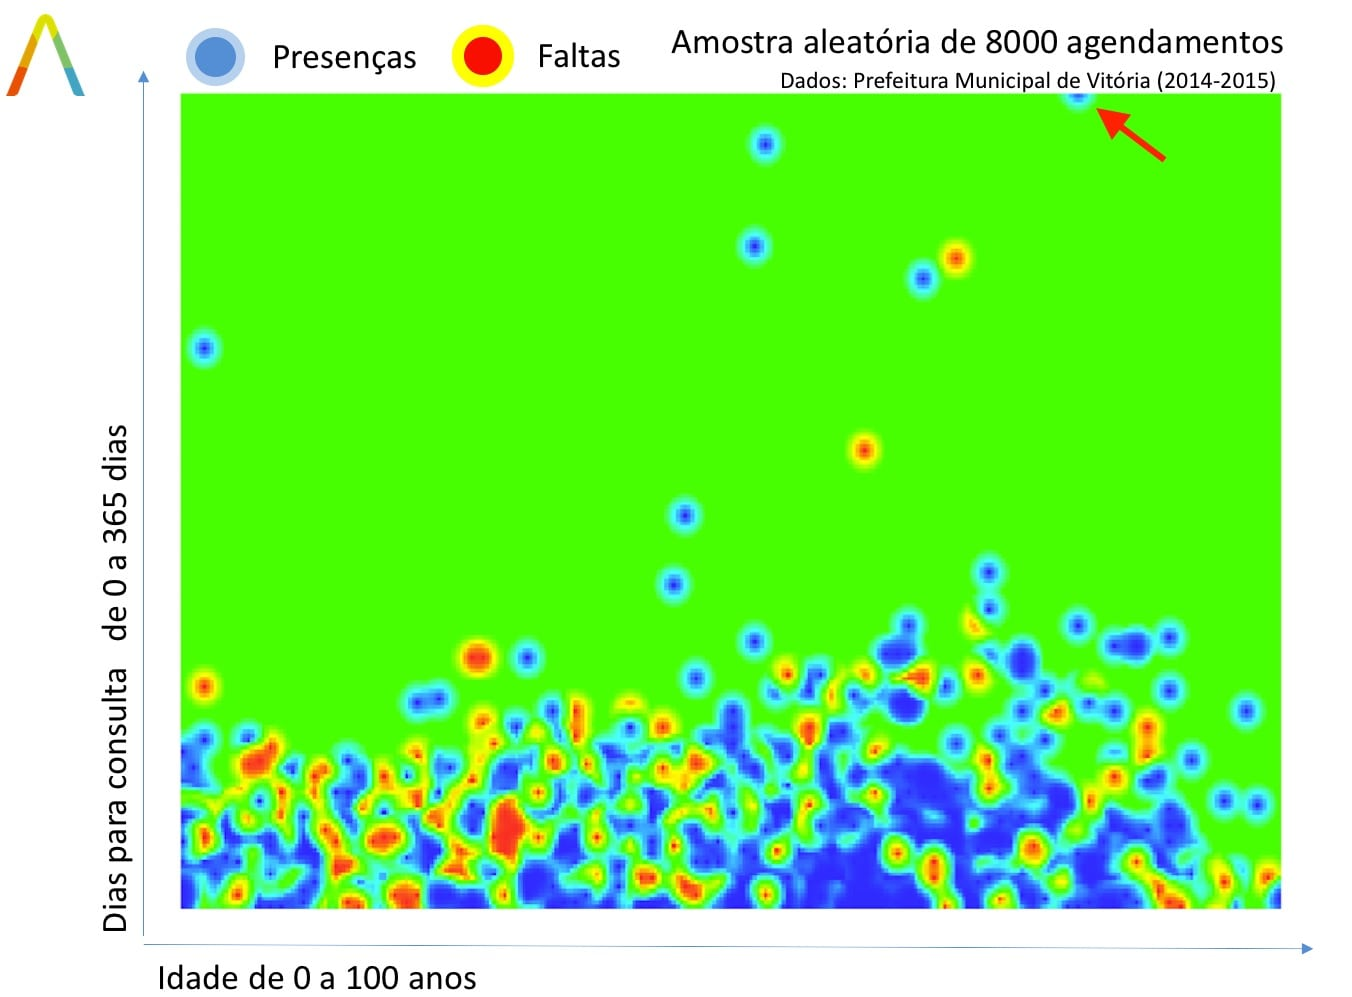
\includegraphics[width=0.7\linewidth]{G:/Hiro/Documents/Meus feitos/Livro ML/bookdown-demo-master/Figuras/outlier} 

}

\caption{``Gráfico de estudo no sistema de saúde apresentando \emph{outlier} \citep{aquarela}.''}\label{fig:outlier}
\end{figure}



Por diversos motivos pode ocorrer de ter presença de \emph{outlier} nos dados e podem viesar negativamente todo resultado de uma análise e seu comportamente pode muitas vezes ser o que justamente o pesquisador está procurando. Há possibilidade do \emph{outlier} ser importante para o pesquisador entender o por que da anomalia estar acontecendo, ou para identificar algum dado extraído erroneamente, por exemplo.

Uma maneira mais complexa e muito precisa, é de identificá-los através de análise dos dados. Encontrando a distribuição estatísticas que mais e aproxima à distribuição dos dados e utilizar métodos estatísticos para detectar as anomalias. Como por exemplo o uso de histograma e a distribuição normal para verificar os dados que estão dentro e fora do intervalo de confiança (ver \ref{dicio} Distribuição normal).

\hypertarget{transformauxe7uxe3o-de-dados}{%
\section{Transformação de dados}\label{transformauxe7uxe3o-de-dados}}

\hypertarget{tipos-de-datasets}{%
\subsection{\texorpdfstring{Tipos de \emph{datasets}}{Tipos de datasets}}\label{tipos-de-datasets}}

A escolha das medidas estatísticas para sua análise ou modelo de Aprendizado de Máquina dependem muito dos tipos de dados das variáveis em observação. Estes tipos de dados podem ser numéricos (como uma sala de aula, com alunos que variam sua altura de 1,51 metros a 1,98 metros) e categórico (como uma classificação num hospital de pacientes doentes ou não doentes), embora esses dois tipos podem ser subdivididos como números inteiros e ponto flutuante para variáveis numéricas e booleano, ordinal ou nominal para variáveis categóricas.

As subdivisões mais comuns são:
- Variáveis Numéricas:
1. Variáveis inteiras (exemplo: \(1,2,3,..., n\));
2. Variáveis de ponto flutuante (parte fracionária, por exemplo: 1,17; 0,10; 47,2).

\begin{itemize}
\tightlist
\item
  Variáveis categóricas:

  \begin{enumerate}
  \def\labelenumi{\arabic{enumi}.}
  \tightlist
  \item
    Variáveis booleanas (dicotômicas, binárias: Verdadeiro e Falso).
  \item
    Variáveis ordinais (1º, 2º, 3º, etc).
  \item
    Variáveis nominais (não possuem ordenação como por exemplo, cor dos olhos: azuis, castanhos, pretos e verdes).
  \end{enumerate}
\end{itemize}

Importante ressaltar que quando trabalhamos dentro da programação, possuem mais tipos além de \emph{int} (númericos inteiros) \emph{char} (caracteres) e \emph{float} (pontos flutuantes), como o \emph{double} que armazena números com ponto flutuantes com precisão dubla com o dobro da capacidade de \emph{float}, \emph{string} como cadeia de caracteres.

Muitos algoritmos possuem a limitação de trabalhar somente com atributos qualitativos (variáveis categóricas), com isso muitas vezes é necessário aplicar algum método capaz de transformar um atributo quantitativo em um atributo qualitativo (faixas de valores). Uma estratégia que cresce ao longo do tempo é o processo de \textbf{discretização} que transforma atributos contínuos em atributos discretos como por exemplo, dividir alturas entre menor que 1,70 metros e maior igual que 1,70 metros. Dependendo do estudo pode ser adequado, embora o pesquisador precisa tomar muito cuidado pois é provável que possar perder algumas informações. De mesmo modo, é possível transformar variáveis categóricas em númericas, como por exemplo classificar tamanhos como pequeno = 1, médio = 2 e grande = 3 possibilitando por meio do mapeamento manter a ordem dos valores (\citet{batista2003pre}).

É bem comum estes tipos de tratamento de dados ao caso de datas, como trabalhos que aplicam-se \textbf{séries temporais} em que o pesquisador precisa estudar a sazonalidade de algum objeto de estudo. A soja por exemplo pode-se analisar sua tendência ao longo dos anos, mas quando tratamos os dados e analisamos em outro período podemos verificar que possui sazonalidades em sua produção. Em análises para investimentos também, atentar o comportamento mensal e diário das ações de uma empresa, muitas vezes está com tendência de alta num âmbito mensal, porém ao analisar diariamente é possível que esteja em baixa.

Para facilitar a compreensão, considere a série temporal \emph{AirPassengers} que representa o número de passageiros mensalmente em uma empresa de transporte aéreo ao período de 1949 a 1960 \citep{box1976time}.

\begin{figure}

{\centering 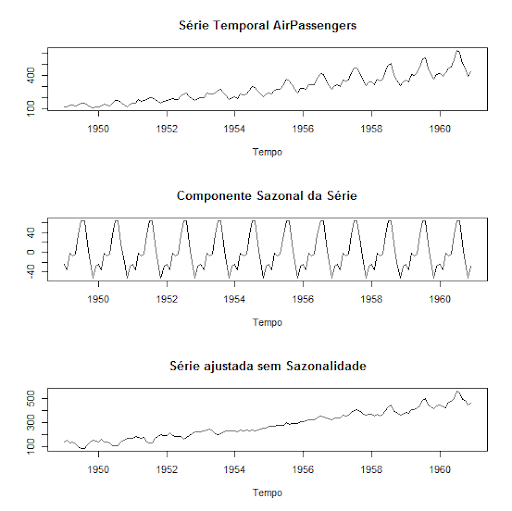
\includegraphics[width=0.7\linewidth]{G:/Hiro/Documents/Meus feitos/Livro ML/bookdown-demo-master/Figuras/airpassengers} 

}

\caption{``Número de passageiros tratados mensalmente \citep{box1976time}.''}\label{fig:airpassengers}
\end{figure}



Para o campo de transformação de dados e séries temporais, ao leitor que pretende ir mais a fundo nestes outros ``galhos'' de estudos. Recomendo buscar outras literaturas que tem como foco este temas. Em discretizações por exemplo, \citet{dougherty1995supervised} e \citet{garcia2012survey} abordam diversos métodos que podem agradá-lo.

\hypertarget{normpadro}{%
\subsection{Normalização e padronização}\label{normpadro}}

Muitos conjuntos de dados apresentam atributos contínuos que espalham-se em diferentes faixas de valores ou possuem distintas variações, devido às suas naturezas ou escalas em que foram medidas. Estas diferenças podem ser fundamentais e precisam ser levadas em conta \citep{carvalho2011inteligencia}. Em situações também para validarmos a análise variância precisa-se dos requisitos de atiditividade, independência, normalidade e homogeneidade de variâncias - será apresentada em ANOVA seção XXXXXXXX. Quando alguma das características mencionadas acontece ou não verifica seus requisitos o pesquisador, antes de fazer uma análise não-paramétrica (\ref{dicio}), pode-se transformar seus dados \citep{banzatto1992experimentaccao}.

\begin{enumerate}
\def\labelenumi{\arabic{enumi}.}
\tightlist
\item
  \textbf{Normalização por reescala:} através de um valor mínimio e um máximo, gera um novo intervalo onde os valores de um atributo estão contidos. Um intervalo entre 0 e 1.
  \begin{equation}
  x_{ij}=\frac{x_{ij}-min_j}{max_j-min_j}
  \label{eq:normalizacao}
  \end{equation}
\end{enumerate}

sendo \(x_i\) a observação de ordem \(i\), \(min_j\) e \(max\) os valores mínimos e máximos do atributo \(j\) respectivamente.

\begin{enumerate}
\def\labelenumi{\arabic{enumi}.}
\setcounter{enumi}{1}
\tightlist
\item
  \textbf{Transformação de raiz quadrada:} frequentemente utilizada para dados de contagens que geralmente segue uma distribuição de Poisson (\ref{dicio}), onde a média é igual à variância \citep{banzatto1992experimentaccao}.
\end{enumerate}

\begin{equation}
\sqrt{x_i}
\label{eq:transraiz}
\end{equation}

sendo \(x_i\) representando as observações do banco de dados. Quando ocorrem zeros ou valores baixos (menores que 10 ou 15), recomenda-se \(\sqrt{x+0,5} \ \mbox{ou} \sqrt{x+1,0}\) \citep{banzatto1992experimentaccao}.

\begin{enumerate}
\def\labelenumi{\arabic{enumi}.}
\setcounter{enumi}{2}
\tightlist
\item
  \textbf{Transformação angular:} recomenda-se para dados expressos em porcentagens, que geralmente seguem a distribuição binomial (\ref{dicio}). Atualmente existe tabelas apropriadas para essa transformação \citep{banzatto1992experimentaccao}. Segundo \citet{banzatto1992experimentaccao} porcentagens entre 30\% e 70\% ou as porcentagens são resultantes da divisão dos valores observados nas parcelas por um valor constante tornam-se desnecessárias e pode-se analisar diretamente os dados originais, mas atente-se pois algumas vezes variar essas exceções de acordo com sua área e pesquisador que a propõe.
\end{enumerate}

\begin{equation}
arc \ sen \sqrt{\frac{x}{100}}
\label{eq:transang}
\end{equation}

\begin{enumerate}
\def\labelenumi{\arabic{enumi}.}
\setcounter{enumi}{3}
\tightlist
\item
  \textbf{Transformação logaritmica:} quando verificada determinada proporcionalidade entre as médias e desvios padrões dos diversos tratamentos. É geralmente utilizada para problemas de assimetria (\ref{dicio}). Em casos, por exemplo, tratamentos com amplitude alta como uma população numerosa que varia de 1.000 a 10.000 indivíduos ou tratamentos de baixa amplitude de 10 a 100 indivíduos. Esta trasformação pode ser útil.
\end{enumerate}

\begin{equation}
log(x) \ \mbox{ou} ln(x)
\label{eq:translog}
\end{equation}

Uma vez transformados os dados em logaritmos, a soma de dados logarítmicos não tem o mesmo valor que a soma de seus antilogaritmos, mas representa o produto destes.

\begin{enumerate}
\def\labelenumi{\arabic{enumi}.}
\setcounter{enumi}{4}
\tightlist
\item
  \textbf{Padronização:} é um método muito utilizado por diversas áreas de pesquisa. Neste caso diferentes atributos podem abranger diferentes intervalos, porém possuir os mesmos valores para alguma medida de posição e de variação \citep{carvalho2011inteligencia}. Imagine você como economista interessado em avaliar o desempenho da produção de soja com as variáveis econômicas e monetárias o Brasil e possui as seguintes variáveis: produção de soja anual medida em milhares de toneladas, taxa básica de juros SELIC medida em porcentagem, receita média anual em milhares de reais, área plantada de soja medida em hectares. Já podemos perceber que todos possuem medidas e grandezas bem diferente uma das outras. Este o propósito da padronização, deixar com que todas as variáveis tenham uma medida em comum.
\end{enumerate}

\begin{equation}
x_{ij}=\frac{x_{ij}-\overline{X}}{S_j}
\label{eq:padronizacao}
\end{equation}

em que \(\overline{X_j}\) e \(S_j\) representam a média e o desvio padrão do atributo \(j\) respectivamente. Após a transformação todos os atributos terão a média zero e desvio-padrão unitário.

Caso transformado seu banco de dados e seu banco de dados apresentarem uma distribuição contínua não-normal, ou não-homogênea ou não-aditiva, não há outra alternativa senão utilizar a estatística não-paramétrica.

Resumo geral: Muitos conjuntos de dados apresentam atributos contínuos que espalham-se em diferentes faixas de valores ou possuem variações diferentes, por motivo de suas naturezas ou escalas medidas. Estas diferenças podem ser muito importantes e precisam ser levadas em conta para não causar erros em sua pesquisa. Para isso usam-se alguns métodos para transformar seus dados para que possam ser trabalhados, apresentados os principais neste livro. Em situações para fazermos análise variância precisa-se também ser transformado seus dados caso não cumpra seus requisitos. Caso o problema ainda persistir, precisa-se utilizar estatística não-paramétrica.

\hypertarget{features-selection---seleuxe7uxe3o-de-atributos-sa}{%
\section{Features Selection - Seleção de atributos (SA)}\label{features-selection---seleuxe7uxe3o-de-atributos-sa}}

Uma literatura que achei bastante interessante foi \citet{parmezan2012avaliaccao}. Seguindo sua estrutura a respeito de Seleção de atributos. Podemos definir SA como a determinação de um subconjunto ótimo de atributos, partindo de algum critério ou medida de importância, que representa a informação importante dos dados \citep{parmezan2012avaliaccao}. Extraímos um subconjunto de \(P\) atributos a partir de um conjunto original de \(N\) atributos, sendo \(P\leq M\) \citep{parmezan2012avaliaccao, liu1998feature, lee2005seleccao}. A cada conjunto de dados com \(M\) atributos, existem \(2^M\) subconjuntos de atributos candidatos \citep{langley1994selection}.

Existem diversas metodologias para selecionarmos os atributos que podem variar em sentido de buscas e estratégias para a seleção. Repare que os tópicos mencionados anteriormente também são utilizados para remoção e seleção, foi fragmentado apenas para facilitar a compreensão.

O ``sentido de busca'' influencia na determinação do(S) ponto(s) de partida no espaço de busca, ou seja, na direção em que a busca será realizada e os operadores que serão utilizados. Elas são categorizadas, seguindo \citet{parmezan2012avaliaccao} e \citet{liu2008computational}, em:

• \textbf{Forward Selection - Seleção para Frente:} o estado inicial é estabelecido como vazio (subconjunto vazio de atributos), e os atributos são incluídos um por vez;

• \textbf{Backward Elimination - Eliminação por Trás:} o ponto de partida é iniciado com o conjunto de todos os atributos (completo), tais quais são removidos sucessivamente;

• \textbf{Bidirectional Search - Pesquisa Bidirecional:} como o próprio nome diz, duas buscas são processadas simultâneamente. Ambas terminam quando atingem o centro do espaço de busca, ou quando uma das buscas encontra os melhores atributos antes de alcançar o centro do espaço de busca;

• \textbf{Random Search - Pesquisa Aleatória:} com o propósito de evitar que a busca fique restrita a ótimos locais. Não tem uma direção específica para buscar, pois o ponto de partida da busca e o modo de adicionar ou remover atributos são decididos aleatoriamente.

Além dos sentidos de busca, existem diversas abordagens que avaliam subconjuntos de atributos e que podem remover tanto atributos irrelevantes quanto redundantes \citep{parmezan2012avaliaccao, liu2008computational}. A seguir, as principais abordagens:

• \textbf{\emph{Filter} - Filtro:}

Com a finalidade de filtrar atributos não importantes, essa abordagem é feita antes da construção dos modelos. A ideia é simplesmente receber como entrada o
conjunto de exemplos descrito utilizando somente o subconjunto de atributos importantes identificados. Ela ocorre antes do aprendizado de máquina \citep{john1994irrelevant} e utiliza-se métodos estatísticos diversos para esta seleção, como por exemplo árvores de decisão ou as ``medidas de importância'' que são apresentadas na próxima seção.

• \textbf{\emph{Wrapper}- Empacotar:} ocorre também externamente ao algoritmo de aprendizado. Este método gera um subconjuto candidato de atributos, executa o algoritmo de aprendizado considerado somente esse subcojunto selecionado de treinamento e avalia a precisão desse classificador. Repete-se esse processo para cada subconjunto de atributos até buscar um bom modelo. Como exemplo temos a análise por arvores de decisão e florestas aleatórias (serão apresentadas mais a frente). Tem como desvantagem o custo operacional desta abordagem. Exemplo de aplicações: \emph{Naive Bayes} e Máquina de vetores de suporte para classificação.

• \textbf{\emph{Embedded} - Embutida:} é realizada internamente pelo próprio algoritmo de extração de padrões. Esta estratégia seleciona o subconjunto de atributos no processo de construção do modelo de classificação, durante a fase de treinamento, e geralmente são específicos para um dado algoritmo de aprendizado. A principal diferença dos métodos do tipo \emph{embedded} e \emph{wrapper},
é que em \emph{embedded} depende em relação a um modelo preditivo específico, assim não permite a sua implementação em combinação com outros modelos \citep{souza2014computational}.

Observação e resumo geral: Note que o que muitas vezes confunde o leitor é o excesso de categorias - que ironicamente tem o propósito de organizar e facilitar. Basicamente são estratégias diferentes com sentidos diferentes de se iniciar a busca de atributos que podem ser irrelevantes ou relevantes: antes de criar um modelo de Aprendizado de maquina; usa-se um modelo de aprendizado para selecionar os atributos antes de iniciar uma etapa de análise {[}pode-se até mesmo realizar outro algoritmo de aprendizado após este algoritmo de seleção{]} ou a própria seleção com a análise {[}mesmo algoritmo para selecionar e concluir{]}). Quando misturamos esta estratégia, denominamos de \textbf{híbridos}.

\begin{figure}

{\centering 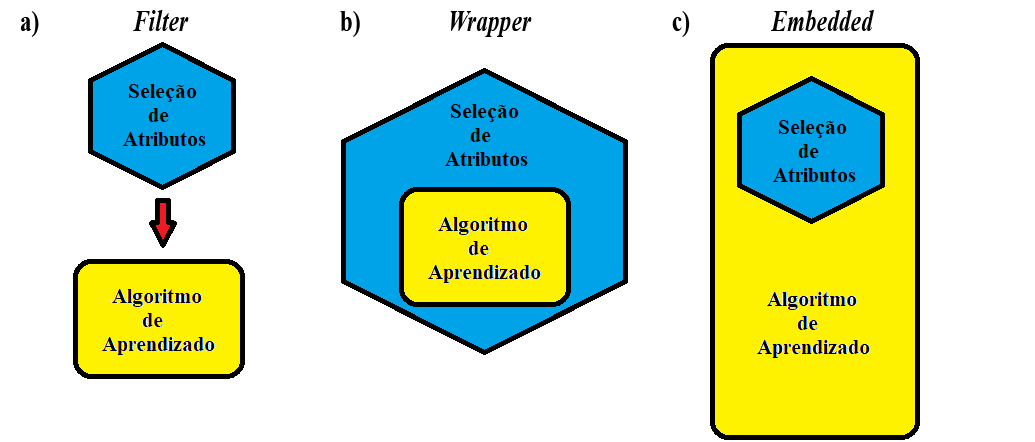
\includegraphics[width=0.7\linewidth]{G:/Hiro/Documents/Meus feitos/Livro ML/bookdown-demo-master/Figuras/diferenssa} 

}

\caption{``Diferença de \emph{Filter}, \emph{Wrapper} e \emph{Embedded} respectivamente (modificado de \citet{covoes2010seleccao}).''}\label{fig:diferenssa}
\end{figure}



\hypertarget{Algoritmosaprendizagem}{%
\chapter{Algoritmos de Aprendizagem - Parte I}\label{Algoritmosaprendizagem}}

\emph{Existe uma infinidade de algoritmos utilizados em machine learning, cada um com uma finalidade específica. Há também características que podem inviabilizar a escolha do modelo mais preciso para determinado problema, como a utilização alto poder computacional.}

Aqui vai a Parte I de Algoritmos de Aprendizagem, neste capítulo serão apresentados:

\begin{enumerate}
\def\labelenumi{\arabic{enumi}.}
\tightlist
\item
  Medidas de Importância:
\end{enumerate}

\begin{itemize}
\tightlist
\item
  Medidas de Informação
\item
  Medidas de Distância
\item
  Medidas de Dependência
\item
  Medidas de Precisão
\item
  Medidas de Consistência
\end{itemize}

\begin{enumerate}
\def\labelenumi{\arabic{enumi}.}
\setcounter{enumi}{1}
\tightlist
\item
  Teste de Hipóteses
\end{enumerate}

\begin{itemize}
\item
\end{itemize}

\begin{enumerate}
\def\labelenumi{\arabic{enumi}.}
\setcounter{enumi}{2}
\item
  Naive Bayes
\item
  Regressão
\end{enumerate}

\begin{itemize}
\tightlist
\item
  Regressão Linear Simples
\item
  Regressão Múltipla
\item
  Modelo de Probabilidade Linear
\item
  Gradiente Descendente
\end{itemize}

\hypertarget{medidas-de-importuxe2ncia}{%
\section{Medidas de Importância}\label{medidas-de-importuxe2ncia}}

\begin{quote}
Um atributo é dito importante se quando removido a medida de importância considerada em relação aos atributos restantes é deteriorada , seja a precisão da medida, consistência, informação, distância ou dependência

Tradução de \citet{liu2012feature}.
\end{quote}

É fundamental estimarmos a importância de um atributo, tanto uma avaliação individual quanto à avaliação de subconjuntos de atributos. É uma questão complexa e multidimensional \citep{liu2012feature}. Podemos avaliar se os atributos selecionados pela etapa do pré-processamento auxiliam a melhorar a precisão do classificador ou a simplifcar algum modelo construído. A seguir, apresenta-se algumas medidas utilizadas \citep{lee2005seleccao}.

\hypertarget{medidas-de-informauxe7uxe3o}{%
\subsection{Medidas de Informação}\label{medidas-de-informauxe7uxe3o}}

As medidas de informação determinam o ganho de informação a partir de um atributo. O ganho de informação é definido como a diferença entre a incerteza a \emph{priori} e a incerteza a \emph{posteriori} considerando-se o atributo \(X_i\). \(X_i\) é preferido ao atributo \(X_j\) se seu ganho de informação for maior que de \(X_j\). Uma das mais utilizadas é a entropia que normalmente é usada na teoria da informação para medir a pureza ou impureza de um determinado conjunto.

\citet{shannon1948mathematical}, tomou como ``ponto de partida'' encontrar uma forma matemática de medir o quanto de informação existe na transmissão de uma mensagem de um ponto a outro, denominando-a entropia. Sua proposta baseava-se na ideia de que o aumento da probabilidade do próximo símbolo diminuiria o tamanho da informação. Com isso, a entropia pode ser definida como a quantidade de incerteza que há em uma mensagem e que diminui à medida que os símbolos são transmitidos (vai se conhecendo a mensagem), tendo-se então a informação, que pode ser vista como redução da incerteza \citep{shannon1948mathematical, paviotti2019consideraccoes}. Por exemplo: ao utilizarmos como idioma a nossa língua portuguesa e ao transmitir como símbolo a letra ``q'', a probabilidade do próximo símbolo ser a letra ``u'' é maior que a de ser qualquer outro símbolo, enquanto que a probabilidade de ser novamente a letra ``q'' é praticamente nula \citep{paviotti2019consideraccoes}.

Shannon define que a entropia pode ser calculada por meio da soma das probabilidades de ocorrência de cada símbolo pela expressão \(∑ p_i = 1 = 100\%\), em que \(p_i\) representa a probabilidade do i-ésimo símbolo que compõe a mensagem. Segundo ele, estes símbolos devem ser representados através de sequências binárias, utilizando das propostas de \citet{nyquist1924certain} e \citet{hartley1928transmission}. Sua proposta consistia em representar símbolos de um alfabeto através de um logaritmo de acordo com suas respectivas unidades de informação. A entropia proposta por ele é obtida pela média das medidas de Hartley \citep{moser2012student}.

Se A é discreto com distribuição de probabilidade \(p(A)\), a entropia será:

\begin{equation} 
  H(A)=- \sum p(A)log_2(p(A)) 
  \label{eq:entropia}
\end{equation}

Para facilitar a compreensão, vamos supor um exemplo de um questionário com resposta binária entre ``sim'' e ``não'': quanto mais distribuído as probabilidades das respostas, mais desorganizada é, logo maior suaa entropia, do contrário caso for uma probabilidade de ser zero ``sim''/``não'' ou de ser 1 (100\%), ou seja, ter apenas uma opção de resposta, será menos distribuído e portanto menor usa entropia.

\begin{figure}

{\centering 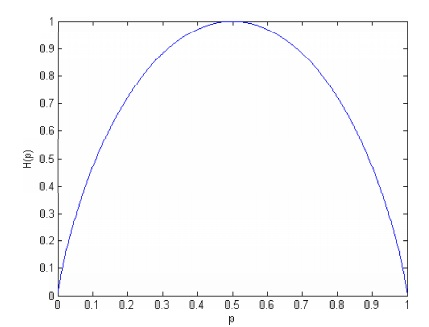
\includegraphics[width=0.7\linewidth]{G:/Hiro/Documents/Meus feitos/Livro ML/bookdown-demo-master/Figuras/entropia} 

}

\caption{Gráfico de Probabilidade x Entropia.}\label{fig:entropia}
\end{figure}



O ganho de informação portanto mede a redução da entropia (nesse caso) causada pela partição dos exemplos de acordo com os valores do atributo.

\begin{equation} 
  \mbox{Ganho de Informação}(D,T)=\mbox{entropia}(D)-\displaystyle \sum_{i=1}^k \frac{|D_i|}{|D|}. \mbox{entropia}(D_i) 
  \label{eq:ganhodeinf}
\end{equation}

É muito utilizado em algoritmo de \textbf{Árvore de decisão} que será apresentado na seção \ref{ptII} mesma seção com um exemplo de seu uso.

\hypertarget{medidas-de-distuxe2ncia}{%
\subsection{Medidas de Distância}\label{medidas-de-distuxe2ncia}}

Também conhecidas com medidas de separabilidade, discriminação e divergência. Em caso de duas classes, um atributo \(X_i\) é preferido ao atributo \(X_j\) se fornece uma diferença maior que \(X_j\) entre as probabilidades condicionais das duas classes. Uma das mais utilizadas é a distância Euclidiana.

\hypertarget{medidasdep}{%
\subsection{Medidas de Dependência}\label{medidasdep}}

\begin{figure}

{\centering 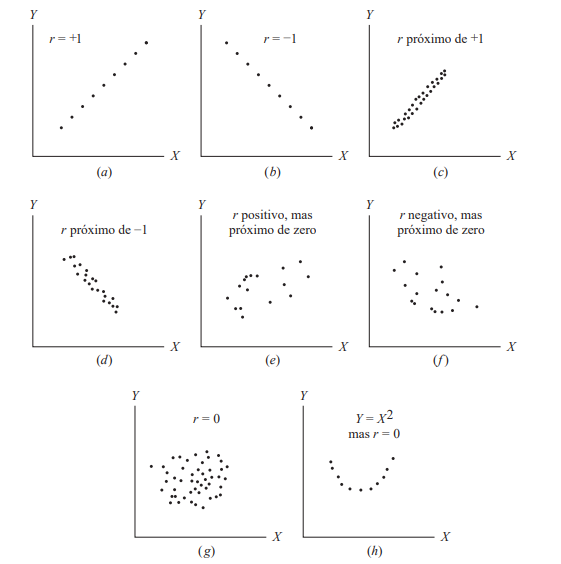
\includegraphics[width=0.7\linewidth]{G:/Hiro/Documents/Meus feitos/Livro ML/bookdown-demo-master/Figuras/correlacao} 

}

\caption{Padrões de correlação. Elaborado por \citet{gujarati2011econometria} e adaptado \citet{theil1978}.}\label{fig:correlacao}
\end{figure}



\hypertarget{medidas-de-precisuxe3o}{%
\subsection{Medidas de Precisão}\label{medidas-de-precisuxe3o}}

\hypertarget{medidas-de-consistuxeancia}{%
\subsection{Medidas de consistência}\label{medidas-de-consistuxeancia}}

\hypertarget{teste-de-hipuxf3teses-e-anuxe1lise-de-variuxe2ncia}{%
\section{Teste de hipóteses e Análise de Variância}\label{teste-de-hipuxf3teses-e-anuxe1lise-de-variuxe2ncia}}

\hypertarget{naive-bayes}{%
\section{Naive Bayes}\label{naive-bayes}}

Antes de falarmos sobre este algoritmo, vamos para o conceito matemático. Em (\ref{dicio}) tratamos do Teorema de Bayes para \(n\) atributos. Colocando-o como probabilidade condicional:

\begin{equation} 
  p(A|B_{1},...,B_{n}) = \\ p(A)p(B_{1}|A)p(B_{2}|A,B_{1}),p(B_{3}|A,B_{1},B_{2})...p(B_{n}|A,B_{1},B_{2},...,B_{n−1})
  \label{eq:bayescond}
\end{equation}

Assumindo que cada atributo \(B_i\) é condicionalmente independente de todos os outros \(B_j\) para \(j\neq i\) e \(p(B_i|A,B_j)=p(B_i|A)\) o modelo poderá ser expresso como:

\begin{equation} 
  p(A_k|B_1,...,B_n)=p(A_k)p(B_1|A_k)p(B_2|A_k),...=p(A_k)\prod_i^n p(B_i|A_k) \ k ∈{1,...,k}
  \label{eq:bayesprodutorio}
\end{equation}

Por fim para podermos classificar, aplicamos argumento de máxima para otimizarmos a função, assim obtém-se o classificador de Naive Bayes:

\begin{equation} 
  \mbox{classificador} \ \hat{y}=argmax \ p(A_k)\displaystyle \prod_{i=1}^n p(B_i|A_k) \ \ k ∈{1,...,k}
  \label{eq:naivebayes}
\end{equation}

Lembrando que para cada atributo, a sua distribuição de probabilidades é assumida como normal.

O Naive Bayes é uma técnica de classificação baseado no teorema de Bayes com uma suposição de independência entre os preditores, ou seja, este classificador assume que a presença de uma característica particular em uma classe não está relacionada com a presença de qualquer outro fator. Por exemplo, uma fruta verde, redonda e com um tamanho de diâmetro X pode ser uma melancia, porém mesmo que estas variáveis dependam uns dos outros e de outras características, todas estas propriedades contribuem de forma independente para a probabilidade de que seja uma melancia. Este modelo é muito utilizado devido que é fácil de construir e particularmente útil para grandes volumes de dados. Porém a própria independência entre os preditores a torna desvantajosa na prática e caso haja variáveis categóricas num conjunto de dados de teste que não forem treinadas, o modelo não irá estimar estas novas variáveis.

\textbf{Exemplo:} para facilitar, podemos supor que estamos trabalhando no diagnóstico de uma nova doença e que foi feito testes em 100 pessoas aleatórias (exemplo de \citet{organica}).

Após coletarmos a análise, descobrimos que das 100 pessoas, 20 possuíam a doença (20\%) e 80 pessoas estavam saudáveis (80\%), sendo que das pessoas que possuíam a doença, 90\% receberam o resultado positivo no teste da doença, e 30\% das pessoas que não possuíam a doença também receberam o teste positivo. Caso uma nova pessoa realizar o teste e receber um resultado positivo, qual a probabilidade de ela realmente possuir a doença?

\begin{figure}

{\centering 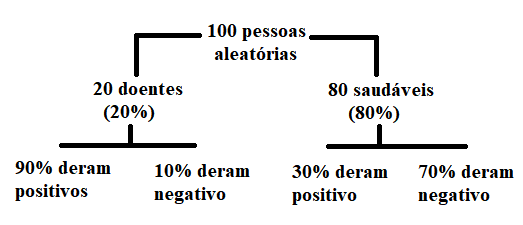
\includegraphics[width=0.7\linewidth]{G:/Hiro/Documents/Meus feitos/Livro ML/bookdown-demo-master/Figuras/bayes} 

}

\caption{Dados coletados de uma amostra de 100 pessoas aleatórias.}\label{fig:bayes}
\end{figure}



Com o algoritmo de Naive Bayes, buscamos encontrar uma probabilidade da pessoa possuir a doença dado que ela recebeu um resultado positivo, multiplicando a probabilidade de possuir a doença pela probabilidade de ``receber um resultado positivo, dado que tem a doença''. De mesmo modo verificar a probabilidade de não possuir a doença dado que recebeu um resultado positivo.

Ou seja, ao caso de ter a doença dado que o resultado deu positivo:
\[P(doença|positivo) = 20\% . 90\% \] \[P(doença|positivo) = 0,2 * 0,9 \] \[P(doença|positivo) = 0,18\]
Para o caso de não ter a doença, dado que deu positivo:
\[P(não \ doença|positivo) = 80\%.30\%\]
\[P(não \ doença|positivo) = 0,8 * 0,3\]
\[P(não\ doença|positivo) = 0,24\]
Após isso precisamos normalizar os dados, para que a soma das duas probabilidades resulte 1 (100\%). Como vimos em pré-processamento \ref{preprocesso}, a \textbf{Normalização por reescala} por meio de um valor mínimio e um máximo, gera um novo intervalo onde os valores de um atributo estão contidos. Um intervalo entre 0 e 1. Portanto, dividimos o resultado pela soma das duas probabilidades.

\[P(doença|positivo) = 0,18/(0,18+0,24) = 0,4285\]
\[P(não doença|positivo) = 0,24/(0,18+0,24) = 0,5714\]
Logo, podemos concluir que se o resultado do teste da nova pessoa for positivo, ela possui aproximadamente 43\% (0,4285) de chance de estar doente.

\textbf{Observação e resumo geral:} Naive Bayes é uma técnica de classificação baseado no teorema de Bayes com uma \textbf{suposição de independência entre os preditores} diferentemente do caso em \ref{dicio} (Teorema de Bayes), ou seja, O Naive Bayes assume que a presença de uma característica particular em uma classe não está relacionada com a presença de qualquer outro fator. Ao caso da melancia, uma fruta verde, redonda e com um tamanho de diâmetro X é possível ser ela, porém mesmo que estas variáveis dependam uma das outras e de outras características, elas contribuem de forma independente para a probabilidade de que seja uma melancia. É um modelo simples de construir e útil para grandes volumes de dados. Porém a própria independência entre os preditores a torna desvantajosa para apliação prática e que variáveis categóricas num conjunto de dados de teste que não foram treinadas, não irá estimar essa nova variável.

Por isso \emph{Naive} vem do significado ``ingênuo'', pois como a Figura \ref{fig:naive} demonstra, os atributos contribuem de forma independente para a probabilidade de A.

\begin{figure}

{\centering 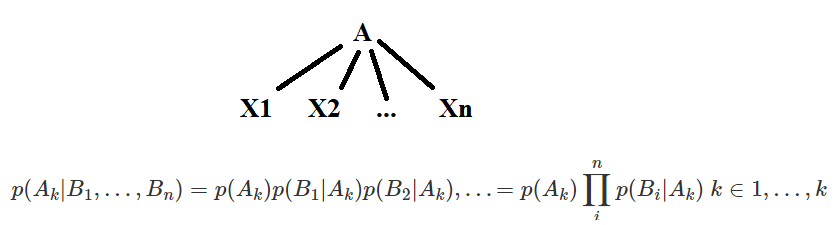
\includegraphics[width=0.7\linewidth]{G:/Hiro/Documents/Meus feitos/Livro ML/bookdown-demo-master/Figuras/naive} 

}

\caption{Gráfico de Probabilidade x Entropia.}\label{fig:naive}
\end{figure}



\hypertarget{reg}{%
\section{Regressão}\label{reg}}

\hypertarget{reglin}{%
\subsection{Análise de Regressão Linear Simples}\label{reglin}}

A análise de variância, pressupõe a independência dos efeitos dos diversos tratamentos utilizados no experimento. Quando a hipótese não é verificada, necessitamos refletir a dependência entre os efeitos dos tratamentos. No caso de experimentos quantitativos, frequentemente justifica a existência da equação de regressão, que une os valores dos tratamentos aos analisados. Em grande parte, trata de estimação e/ou previsão do valor médio (para população) da variável dependente com base nos valores conhecidos da variável explanatória, ela é supervisionada.

Como na prática não conseguimos análisar uma população, trabalhamos em cima de amostras e estimamos para o todo, para que possamos fazer uma aproximação. Partimos da ideia de estimarmos uma função com dados amostrais com o menor erro possível. Portanto, o \(Y_i\) (população) observado pode ser expresso como:

\begin{equation}
    Y_i=\hat{Y_i}+\hat{\mu_i}
    \label{eq:frp}
\end{equation}

E o modelo para função de regressão amostral:
\begin{equation}
    Y_i=\hat{\beta_0}+\hat{\beta_1}X_i+\hat{\mu_i}
    \label{eq:fra}
\end{equation}

em que:

\(\hat{Y_i}\) é o valor observado com \(i\) níveis de \(X\) (estimador da esperança \(E(Y|Xi)\)), \(\hat{\beta_0}\) a constante de regressão estimado e intercepto de \(\hat{Y}\), \(\hat{\beta_1}\) o coeficiente de regressão estimado que seria a variação de \(\hat{Y}\) em função da variação de cada unidade de \(X\), \(X_i\) com \(i\) níveis da variável independente e \(\hat{\mu_i}\) é o erro associado à distância entre o valor observado e o correspondente ponto na curva. Note que os ``chapéis'' em cima das variáveis é utilizado quando referimos a estimações, ou seja, são variáveis de dados amostrais e não a população.

Mas como estimâmetros os parâmetros da função de forma que fique mais próxima possível e com o menor erro? Com o \textbf{Método dos Mínimos Quadrados (MMQ)} atribuído ao Carl Friedrich Gauss - matemático alemão - torna-se possível estimar os melhores \(\beta_0\) e \(\beta_1\) que minimizam os erros.

Como não podemos observar a função de regressão populacional (FRP), precisamos estimálo por meio da função de regressão amostral:
\[Y_i=\hat{\beta_0}+\hat{\beta_1}X_i+\hat{\mu_i} \\ Y_i=\hat{Y_i}+\hat{\mu_i}
\\ \mbox{Logo temos que} \rightarrow \ \hat{\mu_i}=Y_i-\hat{\beta_0}-\hat{\beta_1} X_i\]

Podemos ver que os erros \(\hat{\mu_i}\) (resíduos) são basicamente as diferenças entre os valores observados e estimados de \(Y\). Ao caso de dados com \(n\) pares de observações de \(Y\) e \(X\), queremos encontrar a FRA que se encontra o mais próximo possível do \(Y\) observado, ou seja, escolher a
FRA de modo que a soma dos resíduos \(\sum \hat{\mu}_i=\sum(Y_i-\hat{Y_i})\) seja a menor possível. Porém, como se pode ver pelo diagrama de dispersão na Figura \ref{fig:mmq}, os erros possuem a mesma importância com variações entre sinais positivos e negativos e sua somatória será zero. Isso dificultari a possibilidade de minimizarmos.

\begin{figure}

{\centering 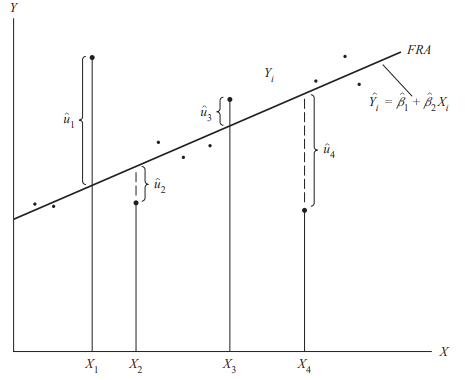
\includegraphics[width=0.7\linewidth]{G:/Hiro/Documents/Meus feitos/Livro ML/bookdown-demo-master/Figuras/mmq} 

}

\caption{Critério do minímos quadrados \citet{gujarati2011econometria}.}\label{fig:mmq}
\end{figure}



Para evitarmos isso, utilizamos o critério dos mínimos quadrados, de modo que elevamos os resíduos ao quadrado. Fazendo isso, o método dá mais peso aos resíduos (não irão mais se anular), podendo visualizar melhor o ``tamanho'' do erro total e obter propriedades estatísticas mais desejáveis.

\begin{equation}
    \sum \hat{\mu}^2_i=\sum(Y_i-\hat{Y_i})^2 \\ = \sum (Y_i-\hat{\beta_0}-\hat{\beta_1})X_i^2 
    \label{eq:mmqeq}
\end{equation}

O método dos mínimos quadrados nos oferece estimativas únicas de \(\beta_0\) e \(\beta_1\) que proporcionam o menor valor possível (encontrando \(\hat{\beta_0}\) e \(\hat{\beta_1}\)) de \(\sum \hat{\mu}_i\). Por meio de cálculo diferenciável (recomendo o leitor interessado em se aprofundar na definição matemática buscar literaturas em foco estatísticoler, como por exemplo a seção 3A de \citet{gujarati2011econometria}) encontra-se:

\begin{equation}
    \sum Y_i=n\hat{\beta_0} + \hat{\beta_1} \sum X_i
    \label{eq:sumyi}
\end{equation}

\begin{equation}
    \sum Y_i X_i=\hat{\beta_0} \sum X_i + \hat{\beta_1} \sum X_i^2
    \label{eq:sumyixi}
\end{equation}

AQUI VOU COLOCAR DO JEITO Q FIZ EM ECONOMETRIA COM AS DEFINCOES E AS DERIVADAS

Para que seja feito o modelo de regressão, ela depende das premissas: independência das variáveis erro, homogeneidade das variâncias, normalidade e relação linear entre as variáveis.

\begin{itemize}
\tightlist
\item
  \textbf{Coeficiente de determinação \(r^2\): medir a qualidade de seu ajuste}
\end{itemize}

Estimamos os parâmetros e o erro da função, agora precisamos considerar a \textbf{qualidade do ajuste} da linha de regressão ajustada a um conjunto de dados, ou seja, vamos descobrir quão ``bom'' o ajuste dessa linha de regressão
amostral é adequada aos dados. Se todas as observações estivessem exatamente em cima da linha de regressão, seria ``perfeito'', o que raramente acontece e provávelmente seria um problema de \textbf{Overfitting} (será apresentado no próximo capítulo para verificarmos a validade do modelo). O coeficiente de terminação \(r^2\) é um medida que diz quanto a linha de regressão
amostral ajusta-se aos dados.

Para entendermos melhor, vamos visualizar por Diagrama de Venn \citep{kennedy1981ballentine}. O círculo \(Y\) representa a variação da variável dependente \(Y\) e o círculo \(X\), a variação da variável explanatória \(X\) como vimos em regressão linear. A área sombreada indica o quanto em que a variação de \(Y\) é explicada pela variação de \(X\). Quanto maior a área sobreposta, maior a parte da variação de \(Y\) é explicada por \(X\). O coefiente de determinação \(r^2\) é apenas a medida numérica dessa sobreposição. Na Figura \ref{fig:ballentine}, conforme move-se da esquerda para a direita, a sobreposição aumenta, ou seja, uma proporção cada vez maior da variação de \(Y\)
é explicada por \(X\) (o \(r^2\) aumenta). Sem sobreposição, \(r^2=0\) e com total sobreposição, \(r^2=1\), pois 100\% da variação de \(Y\) é explicada por \(X\). Portanto o coefienciente situa-se no intervalo entre 0 e 1.

\begin{figure}

{\centering 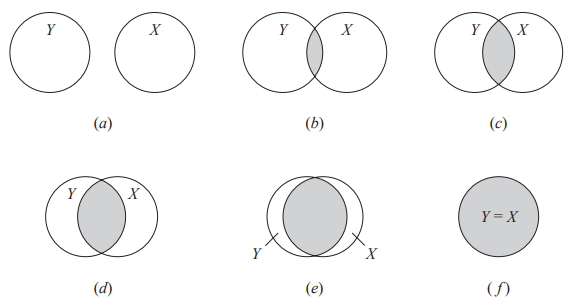
\includegraphics[width=0.7\linewidth]{G:/Hiro/Documents/Meus feitos/Livro ML/bookdown-demo-master/Figuras/ballentine} 

}

\caption{Critério do minímos quadrados \citet{gujarati2011econometria}.}\label{fig:ballentine}
\end{figure}



Podemos chegar ao coeficiente de determinação apenas por manipulação algébrica:

\[\mbox{sabemos que:} \ y_i=\hat{y}_i+\hat{\mu}_i \\
\mbox{elevando ao quadrado e somando a amostra:} \ \sum y^2_i=\sum \hat{y}^2_i+\sum \hat{\mu}^2_i+2\sum \hat{y}_i \hat{\mu}_i \\
\mbox{como} \ \sum \hat{\mu}_i=0, \ \mbox{temos que:}\ \sum y^2_i= \hat{y}^2_i+\sum \hat{\mu}^2_i \\ \sum y^2_i=\hat{\beta}^2_1 \sum x_i^2+\sum \hat{\mu}^2_i \]

\begin{equation}
    \mbox{podemos dizer} \ SQT=SQE+SQR
    \label{eq:sqt}
\end{equation}

sendo SQT a soma total dos quadrados, SQE a soma do quadrados explicados e SQR soma dos quadrados dos resíduos.

\[\mbox{dividindo a equação anterior por SQT:}\\ 1=\frac{SQE}{SQT}+\frac{SQR}{SQT} \\ \mbox{definindo}\ r^2 \ \mbox{como:} \ \frac{SQE}{SQT} \]

\begin{equation}
    \mbox{obtemos:} \ r^2=1-\frac{SQR}{SQT} \rightarrow 1 - \frac{\sum \hat{\mu}_i}{\sum (Y_i - \overline{Y}_i)^2}
    \label{eq:coefdet}
\end{equation}

Por manipulação algébrica, podemos verificar também que \(r^2=\hat{\beta}^2_1(\frac{S^2_x}{S^2_y})\), sendo \(S^2_x\ \mbox{e} \ S^2_y\) as respectivas variâncias amostrais de \(X\) e \(Y\).

Note que ao aplicarmos a raiz quadrada no coeficiente de determinação obtemos o coeficiente de correlação visto em \ref{medidasdep}, que mede o grau de associação entre duas variáveis.

\[r=\pm \sqrt{r^2}\]

AQUI VOU COLOCAR UM EXEMPLO DE REGRESSOA PARA ENTENDER E PARTE MATEMATICA e falar de ANOVA

\textbf{Não esqueça:} dependendo das variáveis em estudo é possível que haja comportamento polinomial ao observarmos no gráfico, podendo ser quadrática, cúbica, etc. Os procedimentos são os mesmos de que linear, mas basicamente incluímos a variável e seu respectivo grau. Dependendo do comportamento muitas vezes é mais fácil ao invés e manter em exponencial (não linear), linearizarmos a função por meio dos logaritmos, semi-logaritmicos entre outros. Isso faz com que temos menos trabalho para tratarmos e estimarmos os parâmetros da função exponencial.

\begin{figure}

{\centering 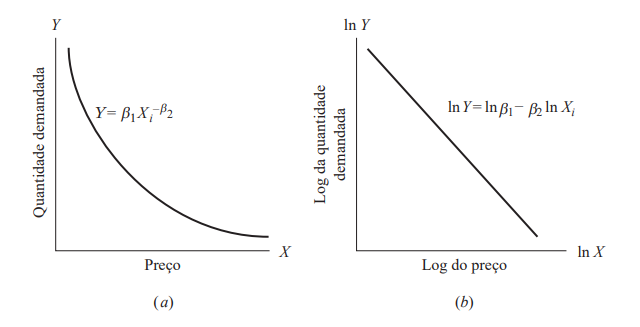
\includegraphics[width=0.7\linewidth]{G:/Hiro/Documents/Meus feitos/Livro ML/bookdown-demo-master/Figuras/explog} 

}

\caption{Em (a) curva de função exponencial e (b) após aplicarmos o logaritmo \citep{gujarati2011econometria}.}\label{fig:explog}
\end{figure}



Atualmente é bem comum utilizarmos o modelo \textbf{log-log}, pois seu coeficiente angular \(\beta_i\) mede a \textbf{elasticidade} de \(Y\) em relação a \(X\), ou seja, a variação percentual de \(Y\) correspondente a uma variação percentual em \(X\). Por exemplo: na Figura \ref{fig:explog} se \(Y\) representa a quantidade demandada de camisetas e \(X\) seu preço unitário. Em (a) temos a relação da quantidade de demanda por camisetas e o preço, mas com a transformação logaritmica teremos a estimação de \(-\beta_2\) (pois é uma reta descendente) que indica a elasticidade preço (variação em \(ln(Y)\) por unidade de variação em \(ln(X)\)). Portanto teríamos a variação percentual da quantidade demandada de camisetas dada uma variação percentual do preço. Atente-se: \textbf{porcentagem} \citep{gujarati2011econometria}.

Resumo geral: Em palavras, r2 mede a proporção ou percentual da variação total de Y explicada pelo modelo de regressão.

\hypertarget{regmult}{%
\subsection{Regressão Linear Múltipla}\label{regmult}}

Na prática deparamos com muitas outros fatores que podem influenciar em sua variável dependente \(Y\). Portanto são acrescentadas dentro de seu modelo de regressão mais variáveis, o que é conhecido como \textbf{Regressão Linear Múltipla}, nada mais do que uma ampliação da regressão linear simples. Num modelo, por exemplo, com três variáveis (caso mais simples) pode ser expressa para a amostra como:

\begin{equation}
    Y_i=\hat{\beta_0}+\hat{\beta_{1}}X_{1i}+\hat{\beta_{2}}X_{2i}+\mu_i
    \label{eq:regmult}
\end{equation}

Da mesma forma, \(Y_i\) a variável dependente, \(X_{2}\) e \(X_{3}\) as independentes explanatórias (explicativa), \(\mu_i\) o erro estocático e \(i\) para indicar \(i\)-ésima observação. Ao caso dos parâmetros, \(\beta_0\) como intercepto, \(\beta_1\) e \(\beta_2\) os \textbf{coeficientes parciais de regressão/angulares}. \(\beta_2\) mede a variação no valor médio de \(Y\) (esperança de \(Y\)), por unidade de variação em \(X_2\), mantendo \(X_3\) constante, ou seja, traz o efeito ``direto'' de uma unidade de variação em \(X_2\) sobre o valor médio de \(Y\), excluindo o efeito de \(X_3\) na média de \(Y\). De mesmo modo, \(X_3\) com \(X_2\) constante.

A regressão múltipla pressupõe as mesma hipóteses de que a regressão linear simples, porém como acréscimo - e muito importante- que as variáveis independentes devem estar \textbf{ausentes de multicolinearidade}, ou seja, não devem haver relação linear entre si. Se essa relação linear existir entre \(X_2\) e \(X_3\) \textbf{são colineares} ou \textbf{linearmente dependentes}, do contrário \textbf{linearmente independentes}. Caso a multicolinearidade for perfeita, os coeficientes de regressão das variáveis \(X\) serão indeterminados e seus erros padrão, infinitos. Se a multicolinearidade for menos que perfeita, serão determinado mas com grandes erros padrão (em relação aos próprios
coeficientes), o que trará um modelo ruim para sua estimação.

Para medirmos a multicolinearidade é comum a análise de \textbf{correlação de pearson} entre todas as variáveis, como mencionada em \textbf{Medidas de Dependência \ref{medidasdep}}, ou analisar a ocorrência de intervalo de confiança mais amplo, verificação de razões ``t'' insignificantes mesmo que seu \(R^2\) esteja alto, parâmetros estimados muitos sensíveis a qualquer alteração de dados e comumente utilizado para verificar o \textbf{fator de inflação de variância (FIV)} \citep{montgomery2012introduction}, que pode ser expressa como:

\begin{equation}
    VIF_j=\frac{1}{1-r^2_j} \ \ j=1,2,...,p
    \label{eq:vif}
\end{equation}

sendo \(r^2\) o coeficiente de correlação ao quadrado e \(j\) para referir as variáveis. Por exemplo, se \(r^2_{23}\), refe-se ao coeficiente de correlação entre as variáveis \(X_2\) e \(X_3\). Segundo ,quando este indicador apresenta o valor acima de cinco, é possível a existência de multicolinearidade \citep{maroco2014analise}.

De mesmo modo que em regressão linear simples, são estimados os MQO, Máxima verossimilhança e o \textbf{coeficiente de determinação múltiplo \(R^2\)} (mesma interpratação para regressão linear simples \(r^2\)) para que se obtenha a melhor aproximação possível.

\hypertarget{mpl}{%
\subsection{Modelo de Probabilidade Linear (MPL)}\label{mpl}}

Considerando um modelo típico de regressão linear simples:
\[Y_i=\beta_0+\beta_1 X_i+\mu_i \]

em que \(X =\)sua renda e \(Y=1\) de que você compre um celular e \(0\) não compre. Como o regressando é binário, ou dicotômico, chamamos de probabilidade linear (MPL). Pode ser interpretada como probabilidade condicional de que o evento ocorra dado \(X_i\), isto é, Pr \((Yi = 1 | Xi)\). Neste caso, é a probabilidade de você comprar um celular e cuja renda é dado por \(X_i\).

Para entender este modelo, vamos supor \(E(\hat{\mu}_i)=0\) para evitarmos estimadores tendenciosos (erros). Portanto:

\begin{equation}
    E(Y_i|X_i)=\beta_0+\beta_1 X_i
    \label{eq:regcond}
\end{equation}

Com \(P_i=\)probabilidade de que \(Y_i=1\)(ocorrência do evento) e \((1-P_i)\)=probabilidade de \(Y_i=0\)(não ocorrência do evento). \(Y_i\) possui a seguinte \textbf{distribuição de probabilidade de Bernoulli}:

\begin{longtable}[]{@{}cc@{}}
\toprule
\textbf{\(Y_i\)} & \textbf{Probabilidade}\tabularnewline
\midrule
\endhead
\(0\) & \(1-P_i\)\tabularnewline
\(1\) & \(P_i\)\tabularnewline
\textbf{Total} & \(1\)\tabularnewline
\bottomrule
\end{longtable}

Aplicando a esperança, obtemos:

\begin{equation}
    E(Y_i)=0(1-P_i)+1(P_i)=P_i
    \label{eq:esperbernoulli}
\end{equation}

Igualando \eqref{eq:esperbernoulli} com \eqref{eq:regcond}, obtemos:

\begin{equation}
    E(Y_i|X_i)=\beta_0+\beta_1 X_i
    \label{eq:regprob}
\end{equation}

Isso verifica que a esperança condicional do modelo de regressão \eqref{eq:frp} pode ser interpretada como a probabilidade
condicional de \(Yi\). Note que, como explicado em \ref{dicio} sobre \textbf{Distribuição Bernoulli} e \textbf{Distribuição Binominal}, caso haja \(n\) observações independentes, cada um com uma probabilidade \(p\) (sucesso) e probabilidade \((1 - p)\) (fracasso) e \(X\) dessas observações representarem o número de sucessos, \(X\) então segue a distribuição binomial (com médi \(np\) e variância \(np(1-p)\). Lembrando que a probabilidade \(P_i\) situa-se entre 0 e 1 \(\rightarrow 0 \leq E(Y_i|X_i) \leq 1\).

Alguns detalhes importantes:

\begin{itemize}
\item
  A hipótese de normalidade de \(\mu_i\) não se verifica no caso dos modelos de probabilidade linear, pois os termos de erro assumem também apenas dois valores, seguindo a distribuição de Bernoulli. Se objetivo for a estimação pontual, a hipótese de normalidade deixa de ser necessária \citep{gujarati2011econometria} e que conforme aumentamos o tamanho da amostra indefinidamente, os estimadores de MQO tendem geralmente a distribuir-se normalmente.
\item
  Como sabe-se, a média e variância de uma distribuição Bernoulli possuem respectivamente \(p\) e \(p(1-p)\). Logo a variância é heterocedástica \(var(\mu_i)=P_i(1-P_i)\) e portanto os estimadores de MQO não são eficientes (não possuem variância mínima). Podemos fazer a transformação para que seja homocedástico:
  \[\sqrt{E(Y_i|X_i)-[1-E(Y_i|X_i)]}=\sqrt{P_i(1-P_i)=\sqrt{w_i}}\]
  \begin{equation}
    \frac{Y_i}{\sqrt{w)i}} = \frac{\beta_0}{\sqrt{w)i}}+\frac{\beta_1 X_i}{\sqrt{w)i}}+\frac{\mu_i}{\sqrt{w)i}}
    \label{eq:probhomecedastico}
  \end{equation}
\end{itemize}

Com a transformação, pode-se calcular por MQO (ponderados).

\textbf{Alternativas para o MPL:}

\begin{itemize}
\item
  Como mencionado, a probabilidade condicional situa-se entre \(0\) e \(1\), porém por MQO não levarem em conta esta restrição. Pode-se verificar os valores que constam entre o intervalo, considerando os valores negativos como \(0\) e maiores que \(1\) como iguais a \(1\) ou aplicar algum outro modelo para garanti-los dentro dos intervalos.
\item
  O \(R^2\) costuma-se situar muito abaixo de 1. Por ser limitado em caso de modelos binários, muitos pesquisadores buscam evitar seu uso.
\end{itemize}

Os modelos mais comuns para ser utilizado como alternativa ao MPL são o \textbf{logit} e o \textbf{probit} para evitar estes problemas.

\hypertarget{logit}{%
\subsubsection{Logit}\label{logit}}

A fim de fazer com que \(P_i\) varie entre 0 e 1 e relacione-se linearmente a \(X_i\), a \textbf{função de distribuição logística} pode ser expressa como:

\begin{equation}
    P_i=\frac{1}{1+e^{-Z_i}}=\frac{e^Z_i}{1+e^Z_i}
    \label{eq:logitpi}
\end{equation}

e \((1-P_i)\) da probabilidade fracasso:

\begin{equation}
    1-P_i=\frac{1}{1+e^{Z_i}}\rightarrow e^{Z_i}
    \label{eq:logitmenospi}
\end{equation}

onde \(Z_i=\beta_0+\beta_1X_i\). Assim \(Z_i\) varia de \(-\infty\) a \(\infty\) e portanto \(P_i\) entre 0 e 1.

Para estimarmos a MQO, precisamos linearizar a função:

\begin{equation}
    L_i=ln(\frac{P_i}{1-P_i})=Z_i=\beta_0+\beta_1 X_i
    \label{eq:logitlinear}
\end{equation}

O modelo \textbf{logit} faz com que:

\begin{itemize}
\item
  A probabilidade varie entre 0 e 1, enquanto \(Z\) e \(L\) possam variar de \(-\infty\) a \(\infty\);
\item
  Mesmo que as probabilides não sejam lineares, \(L\) é linear em \(X\);
\item
  Pode-se aplicar com mais regressores e com mesma interpretação angular medindo a variação de \(L\) para uma unidade variação em \(X\) e para o intercepto;
\item
  Se \(L\) torna-se maior e positivo quando as chances do evento de interesse ocorrer aumenta, do contrário (maior e negativo) de não ocorrer;
\item
  Como em MPL, o modelo Logit é heterocedástico precisa-se ponderar \citep{gujarati2011econometria, cox1970analysis}:
  \begin{equation}
    \sqrt{w_i}L_i=\beta_0 \sqrt{w_i}+\beta_1\sqrt{w_i}X_i+\sqrt{w_i}\mu_i 
    \label{eq:mqplogit}
  \end{equation}
\end{itemize}

em que, com a variância \(\hat{\sigma}^2=\frac{1}{N_i\hat{P_i}(1-\hat{P_i})}\), \(W_i\) é o peso \(N_i\hat{P_i}(1-\hat{P_i})\). Por fim, aplicar o mínimos quadrados ponderados (da mesma forma que MQO, porém com a nova transformação de dados) e estimarmos os parâmetros normalmente.

Como o \(R^2\) não é significativa nos modelos binários. É comum utilizar as \textbf{pseudo \$R\^{}2} {[}long1997regression{]} - existe uma variedade delas - ou o \textbf{Count \(R^2\)} que nada mais é que o número de previsões corretas com o número total de observações. Para a hiótese nula de que todos os coeficientes angulares são simultâneamente iguais a zero, utiliza-se a \textbf{estatística da razão de verossimilhança} que segue a distribuição \(\chi^2\) que equivale ao teste F.

\hypertarget{probit}{%
\subsubsection{Probit}\label{probit}}

\hypertarget{tobit}{%
\subsubsection{Tobit}\label{tobit}}

\hypertarget{exemplo1reg}{%
\subsection{Exemplos}\label{exemplo1reg}}

\hypertarget{GD}{%
\section{Gradiente Descendente (GD)}\label{GD}}

Para a obtenção dos parâmetros de forma analítica, como regressões, muitas vezes é difícil obter os parâmetros que minimizam determinada função de interesse. Dificuldades em obter a solução do sistema na forma fechada (ou não existir) ou quando \(n\) é muito grande, o cálculo da inversa (estimando os parâmetros matricialmente) pode ser muito caro computacionalmente.

O \textbf{Gradiente Descendente (GD)} pode ser muito útil dependendo da situação, conhecido também como \textbf{máximo declive}, é um método númerico utilizado em otimização. Tem como finalidade identificar um mínimo local de uma função de modo iterativo, no qual a cada iteração toma-se a direção do gradiente. Muitas vezes serve como base para algoritmos de segunda ordem como Métodos de Newton, por exemplo.

É uma função para casos gerais, por praticidade vamos supor que temos uma função denominada custo com apenas dois parâmetros \(J(\theta_0,\theta_1)\) e queremos estimar seus parâmetros que minimizam seus erros. Inicialmente atribuímos quaisquer estimativas iniciais para valores de \(\theta_0\) e \(\theta_1\), com o GD vamos alterandos os valores dos \(\theta's\) para reduzirmos \(J(\theta_0,\theta_1)\) até que se chegue a um valor mínimo local.

Um exemplo que gosto muito, por \citet{andrewcoursera}: observe a Figura \ref{fig:gd} e imagine que você está em um campo, com dois montes. Mantenha sua imaginação de que está situado na cruz preta - ponto 0 - no primeiro monte vermelho. Com o GD vamos olhar 360 graus ao redor do ponto em que você está situado apenas para descobrir a resposta de que ``se você fosse dar um pequeno passo em alguma direção ao seu redor com o objetivo de ir para o ponto mais baixo do campo o mais rápido possível, para qual direção você deve andar?''

Supondo que após olhar para todos os lados, com análise de GD você descobriu que seu primeiro passo será no ponto 1 da Figura \ref{fig:gd}. Após isso, você observa novamente para todos os lados e faz outra análise de GD para verificar aonde você vai se deslocar em seu segundo passo para chegar o mais rápido possível até concluir que será o ponto 2. Assim, sucessivamente, você vai se deslocando para os respectivos pontos 3, 4 e sucessivamente até convergir em seu objetivo Z, porém caso você iniciasse pelo ponto K, é bem possível que por meio do GD você descesse o monte por outro trajeto, encontrando outros pontos ótimos locais até chegar a outro ponto otimizado (descer por completo o monte). Esta é a ideia do Gradiente Descendente, por meio de iterações, o algoritmo vai identificando os pontos ótimos (estimadores mínimos) até convergir num ótimo local da função.

Em caso de funções simples como regressão linear, não é necessário o uso de GD. Mas em casos com muitas variáveis e ordens, pode ser bem viável.

\begin{figure}

{\centering 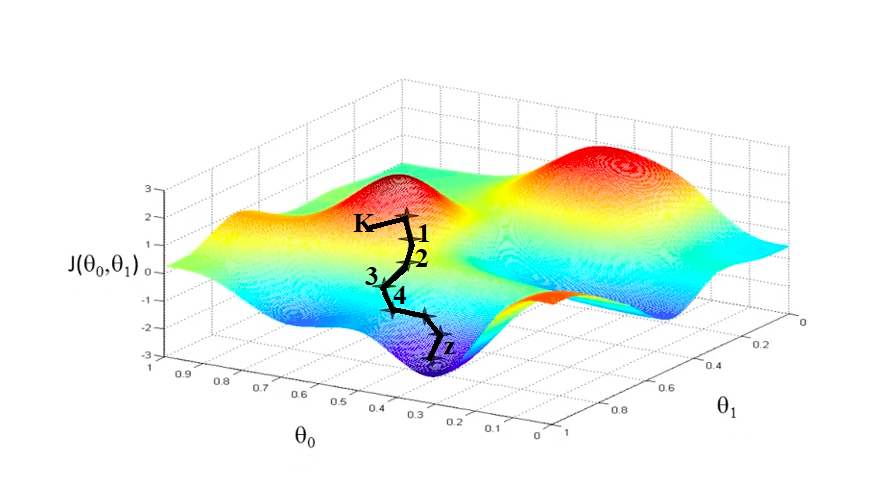
\includegraphics[width=0.7\linewidth]{G:/Hiro/Documents/Meus feitos/Livro ML/bookdown-demo-master/Figuras/gd} 

}

\caption{Gráfico tridimensional a exemplo de Gradiente Descendente \citep{andrewcoursera}.}\label{fig:gd}
\end{figure}



O algoritmo pode ser expresso como:

\begin{equation}
    \theta_j := \theta_j - \alpha \frac{d}{d \theta_j}J(\theta_0,\theta_1) \ \mbox{com} \ j=\theta_0 \ \mbox{e} \ j=\theta_1 
    \label{eq:GD}
\end{equation}

com \(j\) referindo-se à quantidade de observações (parâmetros que pretendemos estimar) da amostra.

O algoritmo é processado da seguinte forma: imagine na mesma Figura \ref{fig:gd} que você irá dar seu primeiro passo, olhou os 360 graus e inseriu as variáveis em seu algoritmo de GD e seu destino é em \(Z=10\). Seu algoritmo calcula se você passou seu destino mais do que devia ou se você está atrás de \(Z\) ainda e também verifica se precisa dar passos grandes por estar bem longe de seu destino, ou passos menores. Supondo que seu \(\alpha\) um pouquinho alto, podemos dar um passo grande para descer o monte (1) pela diferença da observação que você inseriu com \(\alpha \frac{d}{d \theta_j}J(\theta_0,\theta_1)\). Caso fosse uma taxa pequena de \(\alpha\), seu passo seria menor e sua derivada (taxa de variação) vai lhe dizer se você passou do ponto ótimo de \(Z\) (o quão a frente) ou está para trás (quão para trás) desse ponto ótimo.

Com o primeiro passo dado (supor passo \(1 = 40\)), você precisa fazer o mesmo procedimento tomando agora o passo 1 como se fosse o inicial novamente, ou seja, atualizando sua função para cada \(\theta\) \textbf{simultâneamente} (caso dois \(\theta\)'s de entrada para a função, atualiza-se para ambos) até encontrar o novo valor ótimo do próximo passo no ponto \(2=15\). Conforme vai se aproximando de \(Z\), seus passos vão ficando cada vezes menores ( de 15 para 11; de 11 para 10,50; de 10,50 para 10,10; de 10,10 para 10,05; etc) até chegar na melhor aproximação de \(Z=10\) que é o ponto ótimo da função.

Assim o algoritmo encontra os melhores parâmetros para buscar o ponto otimizado, com a estimatiza dos melhores parâmetros para a aproximação com os menores erros (sim! Podemos encontrar os parâmetros dos exemplos de regressão com este algoritmo também!)

Desta forma, atribuímos (``\(:=\)'') para a própria observação de entrada da função receber ela mesma subtraída \(\alpha\) que multiplica a derivada da função em relação a observação de entrada. Para que atualize a cada passo (iteração). \textbf{\(\alpha\)( learning rate - taxa de aprendizagem)} é um valor fixo que controla o tamanho do passo em cada iteração: quando \(\alpha\) for pequeno, o método fica lento, quando grande ele pode falhar na convergência e até mesmo divergir. Seu valor depende muito da pesquisa e de suas fundamentações teóricas, o que recomendo o leitor quando utilizar este método verificar um valor adequado, pode ser que dependendo do valor da taxa demore muito para finalizar o algoritmo pela quantidade de iterações (tamanhos de passos muito pequenos) ou divergir (tamanho de passos muito grandes). \citet{rendle2008online} divulgaram que a fatoração de matrizes para a predição de \emph{ratings} nos dados do desafio \emph{Netflix} precisou de 200 iterações, usando uma taxa de aprendizagem de 0,01.

Para facilitar a compreensão do efeito da taxa de variação, observe a Figura \ref{fig:gd1}. No primeiro gráfico você inicia seu algoritmo com o valor \(\theta\) e com a derivada podemos observar que inclinação da reta tangente ao ponto é positiva (\(\frac{d}{d\theta}j(\theta)\geq 0\)), portanto em \(\theta=\theta-\alpha.\mbox{um valor positivo}\), faz que com que esse novo \(\theta\) (segunda iteração) seja menor que o da primeira iteração, visto que terá que subtrair e deslocar-se para esquerda para tender ao ponto mínimo. Da mesma forma, ao segundo gráfico, podemos verificar que a inclinação é negativa (\(\frac{d}{d\theta}j(\theta)\leq 0\)), portanto \(\theta=\theta-\alpha.\mbox{um valor negativo}\), fará com que o novo \(\theta\) seja maior do que da primeira iteração, pois irá somar e deslocar-se para direita tendendo ao ponto mínimo.

\begin{figure}

{\centering 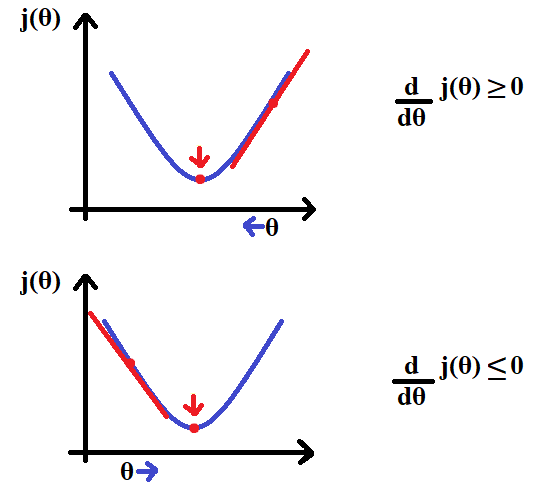
\includegraphics[width=0.7\linewidth]{G:/Hiro/Documents/Meus feitos/Livro ML/bookdown-demo-master/Figuras/gd1} 

}

\caption{Efeito da taxa de variação no Gradiente Descendente.}\label{fig:gd1}
\end{figure}



Como pode-se perceber, a taxa de aprendizagem e a taxa de variação são fundamentais e complementares para o algoritmo de GD, pois elas dizem o tamanho do passo e em que posição estamos em relação ao ponto ótimo da função.

\hypertarget{exemplos}{%
\subsection{Exemplos}\label{exemplos}}

\begin{enumerate}
\def\labelenumi{\arabic{enumi}.}
\tightlist
\item
  \textbf{Uma variável:}Vamos supor a seguinte função custo:
\end{enumerate}

\[j(\theta)=\theta^2\]

Queremos minimizá-la \(min \ j(\theta)\). Portanto precisamos inicialmente colocar um número aleatório para nosso parâmetro - não ótimo - para que o algoritmo atualize a cada iteração. Vamos supor a taxa de aprendizagem (\emph{learning rate}) \(\alpha=0,1\) e \(\theta=4\) para facilitar. Ou seja, \(j(\theta)=4^2=16\). Vamos atualizar os parâmetros:

\[\theta := \theta-\alpha.\frac{d}{d\theta}j(\theta) \\ 
\mbox{derivando a função} \ j(\theta)=\theta^2 \ \mbox{e substituindo:}
\\ \theta:= \theta -\alpha.2\theta \\ \mbox{substituindo os valores de}\ \alpha\ \mbox{e}\ \theta: \\ \theta:=4-0,1 \ .\ 2\ .\ 4 \\
\rightarrow \theta:=3,2\]

Na iteração obtemos \(\theta=3,2\). Se subsituirmos em \(j(\theta)\) novamente, iremos obter \(j(\theta)=(3,2)^2=10,24\). Agora atualizando novamente para a próxima iteração:
\[\theta:= \theta -\alpha.2\theta \\ \theta:=3,2-0,1\ .\ 2\ .\ 3,2 \\
\theta:= 2,56\]

Portanto, \(j(\theta)=(2,56)^2=6,55\). Sucessivamente, vamos fazendo as iterações até convergir:

\begin{longtable}[]{@{}cc@{}}
\toprule
\textbf{\(\theta\)} & \textbf{\(j(\theta)\)}\tabularnewline
\midrule
\endhead
4 & 16\tabularnewline
3,2 & 10,24\tabularnewline
2,56 & 6,55\tabularnewline
2,04 & 4,19\tabularnewline
1,632 & 2,663\tabularnewline
. & .\tabularnewline
. & .\tabularnewline
. & .\tabularnewline
0 & 0\tabularnewline
\bottomrule
\end{longtable}

Da mesma forma, se iniciarmos o algoritmo com -4:

\begin{longtable}[]{@{}cc@{}}
\toprule
\textbf{\(\theta\)} & \textbf{\(j(\theta)\)}\tabularnewline
\midrule
\endhead
-4 & 16\tabularnewline
-3,2 & 10,24\tabularnewline
-2,56 & 6,55\tabularnewline
-2,04 & 4,19\tabularnewline
-1,632 & 2,663\tabularnewline
. & .\tabularnewline
. & .\tabularnewline
. & .\tabularnewline
0 & 0\tabularnewline
\bottomrule
\end{longtable}

Note que conforme \(\theta\) diminui, o custo também. Conforme mais iterações são aplicadas, mais ``ótimo'' será. Graficamente para -4 em vermelho e +4 em azul:

\begin{figure}

{\centering 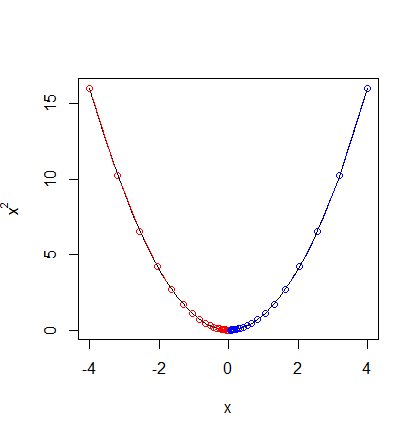
\includegraphics[width=0.7\linewidth]{G:/Hiro/Documents/Meus feitos/Livro ML/bookdown-demo-master/Figuras/gdx2} 

}

\caption{Função \(X^2\) com valores de entrada -4 e +4.}\label{fig:gdx2}
\end{figure}



\begin{enumerate}
\def\labelenumi{\arabic{enumi}.}
\setcounter{enumi}{1}
\tightlist
\item
  \textbf{Duas variáveis:} Vamos supor a seguinte função de custo com \(\alpha=0,1\), \(\theta_1=1\) e \(\theta_2=2\):
  \[j(\theta_1,\theta_2)=\theta_1^2+\theta_2^2 \\ 
  j(\theta_1,\theta_2)=1^2+2^2=5\]
  Queremos \(min \ j(\theta_1,\theta_2)\)Como explicado, ao caso de haver mais de um parâmetro precisamos separar atualizar cada um simultâneamente e aplicar derivada parcial em sua função:
\end{enumerate}

\[\theta_1:=\theta_1-\alpha \frac{d}{d\theta_1}j(\theta_1,\theta_2) \ \ \mbox{e}\ \ \theta_2:=\theta_2-\alpha \frac{d}{d\theta_2}j(\theta_1,\theta_2) \\
\mbox{calculando as derivadas parciais de}\ j(\theta_1,\theta_2)=\theta_1^2+\theta_2^2\ \mbox{obtemos:}\\
\frac{d}{d\theta_1}j(\theta_1,\theta_2)=2\theta_1 \ \
\mbox{e}\ \ \frac{d}{d\theta_2}j(\theta_1,\theta_2)=2\theta_2\]

\[\mbox{substituindo:} \\
\theta_1:=\theta_1-\alpha.\ 2\theta_1 \ \ \mbox{e}\ \ \theta_2:=\theta_2-\alpha .\ 2\theta_2 \\
\mbox{inserindo os valores:}\\
\theta_1:=1-0,1.\ 2.\ 1 \ \ \mbox{e}\ \ \theta_2:=2-0,1.\ 2.\ 2 \\
\theta_1:=0,8 \ \mbox{e} \ \theta_2=1,6\]

Portanto após a iteração, temos que \(j(\theta_1,\theta_2)=0,8^2+1,6^2=3,2\). Da mesma forma, para a próxima iteração temos:

\[\theta_1:=0,8-0,1.\ 2.\ 0,8 \ \ \mbox{e}\ \ \theta_2:=1,6-0,1.\ 2.\ 1,6 \\
\theta_1:=0,64 \ \mbox{e} \ \theta_2=1,28\]

Portanto teremos \(j(\theta_1,\theta_2)=0,64^2+1,28^2=2,048\). Assim sucessivamente:

\begin{longtable}[]{@{}ccc@{}}
\toprule
\textbf{\(\theta_1\)} & \textbf{\(\theta_2\)} & \textbf{\(j(\theta_1,\theta_2)\)}\tabularnewline
\midrule
\endhead
1 & 2 & 5\tabularnewline
0,8 & 1,6 & 3,2\tabularnewline
0,64 & 1,28 & 2,48\tabularnewline
. & . & .\tabularnewline
. & . & .\tabularnewline
. & . & .\tabularnewline
0 & & 0\tabularnewline
\bottomrule
\end{longtable}

\begin{enumerate}
\def\labelenumi{\arabic{enumi}.}
\setcounter{enumi}{2}
\tightlist
\item
  \textbf{Erro quadrado médio (Regressão Linear Simples:)} Observe a função de regressão linear:
  \[f_\theta(X)=\theta_0+\theta_1*X\]
\end{enumerate}

A função de custo:
\[j(\theta)=\frac{1}{m}\displaystyle \sum^m_{i=1}(f_\theta(x^i)-y^i)^2\]

Primeiramente vamos encontrar a derivada parcial de \(j(\theta_0,\theta_1)\):
\[\frac{d}{d\theta_0}j(\theta_0,\theta_1=\frac{d}{d\theta_0}(\frac{1}{m}\displaystyle \sum^m_{i=1}(f_{\theta}(x^i)-y^i)^2) \rightarrow \frac{2}{m}\displaystyle \sum^m_{i=1}(f_\theta(x^i)-y^i) \\
\frac{d}{d\theta_1}j(\theta_0,\theta_1=\frac{d}{d\theta_1}(\frac{1}{m}\displaystyle \sum^m_{i=1}(f_{\theta}(x^i)-y^i)^2) \rightarrow \frac{2}{m}\displaystyle \sum^m_{i=1}(f_\theta(x^i)-y^i)x^i\]
Pode-se também multiplicar a função de custo por \(\frac{1}{2}\) para que quando faz-se a derivada, facilite no cálculo e multiplicar a função de custo por um escalar não irá afetar a localização do mínimo.
\[j(\theta)=\frac{1}{2m}\displaystyle \sum^m_{i=1}(f_\theta(x^i)-y^i)^2\]
Com isso em foco de minimizarmos, basta aplicarmos o banco de dados de \(X\) e \(Y\) em seu modelo e de seus dois \(\theta's\) de entrada. Repetindo as iterações para atualizar seus valores até a convergência e identificando os parâmetros que se aproximam.

\hypertarget{ptII}{%
\chapter{Algoritmos de Aprendizagem - Parte II}\label{ptII}}

\hypertarget{svm}{%
\section{SVM}\label{svm}}

\hypertarget{uxe1rvores-de-decisuxe3o}{%
\section{Árvores de Decisão}\label{uxe1rvores-de-decisuxe3o}}

\hypertarget{elastic-net}{%
\section{Elastic Net}\label{elastic-net}}

\hypertarget{knn}{%
\section{KNN}\label{knn}}

\hypertarget{k-means}{%
\section{K-means}\label{k-means}}

\hypertarget{anuxe1lise-de-componentes-principais}{%
\section{Análise de Componentes Principais}\label{anuxe1lise-de-componentes-principais}}

A Análise de Componentens Principais, popularmente conhecida como ACP ou PCA (\emph{Principal Component Analysis}), em inglês, foi introduzida por \citet{pearson1901liii} e fundamentada no artigo de \citet{hotelling1933analysis}. É uma \textbf{análise multivariada} que tem como objetivo explicar a estrutura de variância e covariância de um vetor aleatório, composto por \(p\)-variáveis aleatórias, através da construção de combinações lineares das variáveis originais que são chamadas de componentes principais e não correlacionadas entre si \citep{mingoti2007analise}. É uma técnica bastante utilizada em diversas áreas do conhecimento, como a biologia, a agronomia, a zootécnica, a ecologia, a engenharia florestal, a medicina, a economia, entre outras áreas. Muitos sugerem o seu uso quando o volume de dados ou variáveis é grande possibilitando reduzir a dimensão da matriz de dados que compõem o conjunto de variáveis resposta com apenas poucos componentes, ou seja, \(p\) variáveis originais substituídas por \(k\) (sendo \(k < p\)) componentes principais não correlacionadas.

Vamos supor um conjunto de dados em apenas duas dimensões \((x, y)\) e que pode ser plotado em um plano cartesiano. Podemos verificar pelo seu comportamento que possuem alta correlação positiva.

\begin{figure}

{\centering 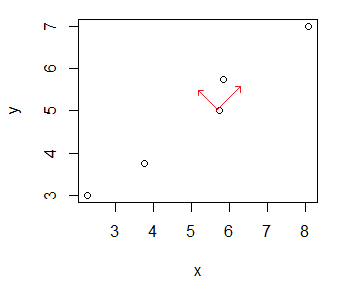
\includegraphics[width=0.7\linewidth]{G:/Hiro/Documents/Meus feitos/Livro ML/bookdown-demo-master/Figuras/pca1} 

}

\caption{Gráfico bidimensional \(x\) por \(y\).}\label{fig:pca1}
\end{figure}



Mas se quisermos descobrir a variação do conjunto de dados, o ACP busca encontrar um novo sistema de coordenadas em que cada ponto tem um novo valor \((x, y)\). Os eixos não representam algo físico, mas representam combinações de \(x\) e \(y\) que denominamos \textbf{``componentes principais''}, escolhidas para analisar a variação do eixo. Observe que rotacionamos o gráfico na Figura \ref{fig:pca2} e que após a ACP, podemos verificar a possibilidade de dercartar a componente referente ao eixo \(y\), visto que a componente do eixo \(x\) explica 99,30\% da variação total dos dados, ou seja, o primeiro componente tem uma maior dispersão (variância). Possibilitando pela componente principal do eixo \(x\), analisar e até mesmo classificar as observações, como por exemplo, a observação 1 e 2 como um conjunto e a 3, 4 e 5 como um segundo conjunto.

\begin{figure}

{\centering 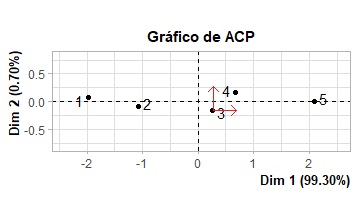
\includegraphics[width=0.7\linewidth]{G:/Hiro/Documents/Meus feitos/Livro ML/bookdown-demo-master/Figuras/pca2} 

}

\caption{Gráfico de \(x\) por \(y\) rotacionado.}\label{fig:pca2}
\end{figure}



Com mais dimensões, o ACP torna-se ainda mais útil pois possibilita observarmos o conjunto de dados num melhor ângulo.

\begin{figure}

{\centering 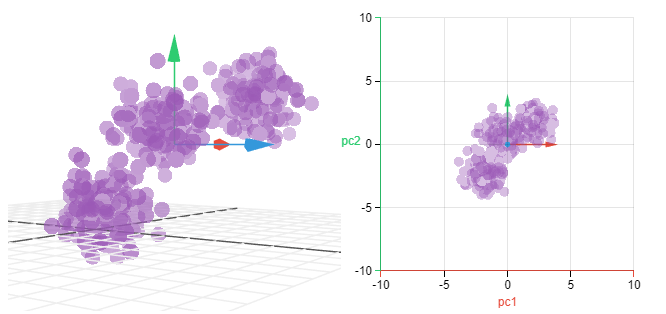
\includegraphics[width=0.7\linewidth]{G:/Hiro/Documents/Meus feitos/Livro ML/bookdown-demo-master/Figuras/pca3} 

}

\caption{Gráfico tridimensional, em \citet{powellpca}.}\label{fig:pca3}
\end{figure}



Portanto, a ACP assume que os dados originais estão representados por características (variáveis) correlacionadas com o objetivo de transformar essas variáveis em novas (componentes principais) por meio de mudança de base do espaço vetorial que não sejam correlacionadas entre si e que estas novas variáveis (menores que as originais) retenha a maior parte da variação apresentada pelas originais, tornando possível a classificação.

A suposição de normalidade não é requisito para sua técnica, mas ainda sim é conveniente padronizar (\ref{normpadro}) cada variável, permitindo que todas as variáveis tenham o mesmo peso para evitarmos viés de escala \citep{hongyu2016analise}. A padronização das variáveis do vetor pelas respectivas médias e desvios padrões, gera novas variáveis centradas em zero e com variâncias iguais a 1. Assim, as componentes principais são determinadas a partir da matriz de covariâncias das variáveis originais padronizadas \citep{mingoti2007analise}.

Agora que sabemos o que é ACP, vamos apresentar alguns conceitos de Álgebra Linear e Estatísticas para compreendermos como é aplicado este método.

\hypertarget{autovalores-e-autovetores}{%
\subsection{Autovalores e Autovetores}\label{autovalores-e-autovetores}}

Caso ainda não tenha muito contato com a Álgebra Linear, recomendo buscar algumas literaturas a respeito. Em \ref{dicio} encontra-se sobre Escalar, Vetores, Espaço Vetorial e Transformação Linear que serão tratadas neste tópico.

Dado uma matriz \(A_{mxn}\) que define uma transformação linear (não muda sua dimensão), existem vetores onde sua orientação não é afetada por esta transformação, os \textbf{autovetores}.

\begin{figure}

{\centering 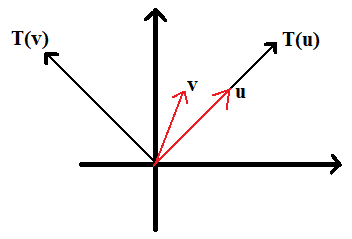
\includegraphics[width=0.7\linewidth]{G:/Hiro/Documents/Meus feitos/Livro ML/bookdown-demo-master/Figuras/autovetor} 

}

\caption{\(u\) é um autovetor de \(T\), porém \(v\) não.}\label{fig:autovetor}
\end{figure}



Um vetor é dito ser autovetor da matriz \(A_{mxn}\) se a transformação linear deste vetor \(T(u)\) é colinear a este vetor, ou seja, \(A_{mxn}\vec{u}=\lambda \vec{u}\). Sendo que \(\lambda\) é um escalar e chamado de autovalor da matriz correspondente ao autovetor. Para encontrarmos o autovetor:

\begin{equation}
    A_{mxn}\vec{u}=\lambda \vec{u} \\
A_{mxn}\vec{u}-\lambda \vec{u}=0 \\
(A_{mxn}-\lambda l)\vec{u}=0
    \label{eq:autovetor}
\end{equation}

esta equação tem solução trivial, ou seja, diferentes da nula \((\vec{v}\neq 0 )\) se e somente se, seu determinante é zero. Conhecido como \textbf{Equação caracterísica} e sua solução são os \textbf{autovalores}:
\begin{equation}
    \mbox{Eq. Característica}\ \  det(A_{mxn}-\lambda l)=0  
    \label{eq:eqcarac}
\end{equation}

Note também que toda transformação linear (matriz) em um espaço
vetorial complexo (números imaginários) tem, pelo menos, um autovetor (real ou complexo).

\hypertarget{exautovetor}{%
\subsubsection{Exemplo}\label{exautovetor}}

\begin{enumerate}
\def\labelenumi{\arabic{enumi}.}
\tightlist
\item
  Vamos considerar um operador linear \textbf{\(T: R^2 \rightarrow R^2\)}. Com \(T(x,y)=(4x+5y,2x+2y)\). Quais são os autovalores a matriz \(A=\begin{bmatrix} 4 &5 \\ 2 &2 \end{bmatrix}\)?
\end{enumerate}

Vamos resolver a equação característica \(det(A_{mxn}-\lambda l)=0\).

\[det(A_{mxn}-\lambda l)=\begin{bmatrix}
4 &5 \\ 
2 &2 
\end{bmatrix} - \lambda \begin{bmatrix}
1 &0 \\ 
0 &1 
\end{bmatrix} = \begin{bmatrix}
4-\lambda &5 \\ 
2 &2-\lambda 
\end{bmatrix}\]

Com \(det(A_{mxn}-\lambda l)=0:\)
\[(4-\lambda)(2-\lambda)-10=0 \\
\lambda^2-6\lambda-2=0 \\ \mbox{resolvendo a equação: } \ 
\lambda_1 \approx 6,32 \  \ \mbox{e} \ \ \lambda_2 \approx -0,32\]

\hypertarget{estatuxedsticas}{%
\subsection{Estatísticas}\label{estatuxedsticas}}

Alguns conceitos de Estatísticas são fundamentais para que se entenda a ACP:

\begin{itemize}
\tightlist
\item
  \textbf{Covariância x Correlação:} como apresentado em \ref{dicio}, a covariância é semelhante à correlação (ver \ref{normpadro}) entre duas variáveis, no entanto, elas diferem que os coeficientes de correlação são padronizados. Isso faz com que um relacionamento linear varie entre \(-1 \leq \rho \leq 1\). A correlação mede tanto a força como a direção da relação linear entre duas variáveis. Ao caso da covariância os valores não são padronizados. Assim, a covariância pode variar de \(-\infty \leq Cov (x,y) \leq \infty\) demonstrando quanto \(x\) e \(y\) mudam juntas. Portanto o valor para uma relação linear ideal depende muito dos dados. Como os dados não são padronizados, é difícil determinar a força da relação entre as variáveis. Note que o coeficiente de correlação é uma função da covariância:
\end{itemize}

\[\rho_{x,y}=\frac{cov(x,y)}{\sigma_x \sigma_y}\]

Uma covariância positiva sempre resulta em uma correlação positiva e uma covariância negativa sempre resulta em uma correlação negativa.

Quando temos um vetor de \(n\) variáveis em vez de apenas duas, iremos obter uma matriz de covariâncias ou correlação. Contendo em sua diagonal a variância \(\sigma^2\), pois \(cov(x_i,x_i)=\sigma^2(x_i)\), por exemplo:

\[\begin{bmatrix}
cov_{1,1} &cov_{1,2=2,1}  &cov_{1,3=3,1} \\ 
cov_{1,1=2,1} &cov_{2,2}  &cov_{2,3=3,2} \\ 
cov_{3,1=1,3} &cov_{2,3=3,2} & cov_{3,3}
\end{bmatrix} = \begin{bmatrix}
var_{1} &cov_{1,2=2,1}  &cov_{1,3=3,1} \\ 
cov_{1,1=2,1} &var_{2}  &cov_{2,3=3,2} \\ 
cov_{3,1=1,3} &cov_{2,3=3,2} & var_{3}
\end{bmatrix}\]

\hypertarget{a-acp}{%
\subsection{A ACP}\label{a-acp}}

Agora que compreendemos alguns conceitos importantes, podemos entender melhor a metodologia da ACP. Assumindo que os dados originais estão representados por variáveis correlacionadas (etapa de pré-processamento), ou seja, não independentes. Vamos ao objetivo de transformar essas \(p\) variáveis em outras novas \(k\) (com \(k<p\)) de ordem decrescesnte de variabilidade e que não sejam correlacionadas e que as primeiras novas variáveis retenham a maior parte da variação apresentadas pelas originais a fim de podermos classificá-los.

Dado um vetor \(\vec{u}\) aleatório com \(p\) variáveis originais. O primeiro componente principal \(y_1\), como dito que deve ser ordem decrescente de variabilidade, será uma combinação linear do vetor \(\vec{u}\) de forma que a variância \(var(y_1)=\sigma^2_{y_{1}}\) seja a máxima (maior possível), ou melhor, precisamos encontrar um vetor \(\vec{\beta^1}\) tal que \(y_1=(\vec{\beta^1})^T \vec{u}\) e \(var(y_1=(\vec{\beta^1})^T \vec{u}\) seja máxima. De mesmo modo para \(y_2\) e um vetor \(\vec{\beta^2}\) e assim sucessivamente para \(p\) variáveis em seu banco de dados.

Ao caso do Exemplo \ref{exautovetor} de Autovalores e Autovetores, foi definida a transformação linear \(T(x,y)=(4x+5y,2x+2y)\) com as duas respectivas componentes \(4x+5y\) e \(2x+2y\). 4 e 5 da primeira componente refere-se, por exemplo, como o vetor \(\vec{\beta^1}\) que multiplicado pelos vetores originais \(x\) e \(y\), temos um novo componente desse novo espaço \(4x+5y\). Da mesma forma à segunda componente \(2x+2y\) com um \(\vec{\beta^2}\).

Para facilitar a compreensão, vamos utilizar um exemplo com duas variáveis (\(R^2\)):
AQUI VOU ARRUMAR E COLOCAR COMO TA EM MINGOTI!
- Queremos encontrar a primeira componente principal \(y_1\), de modo que \(var(y_1)\) seja máxima, ou seja, encontrar um vetor \(\vec{\beta^1}\) tal que \(y_1=(\vec{\beta^1})^T \vec{u}\) e \(var(y_1=(\vec{\beta^1})^T \vec{u}\) seja máxima.

\[var(y_1)=var((\vec{\beta^1})^T\vec{u})=var(\vec{\beta^1_1}\vec{u}_1+\vec{\beta^1_2}\vec{u}_2)\\
= (\vec{\beta^1_1})^2var(\vec{u_1})+(\vec{\beta^1_2})^2var(\vec{u_2})+2\vec{\beta^1_1}\vec{\beta^1_2}Cov(\vec{u_1}\vec{u_2})\\
= (\vec{\beta^1})^TK_{\vec{u}} \vec{\beta^1}\]

Os maiores autovalores são os que orientam o sinal, os demais podem ser descartados. Porém quantos componentes principais devemos utilizar? Precisamos verificar a proporção da variação total dos dados originais que uma componente pode explicar, a partir disso selecionarmos. Lembrando que cada autovalor \(\lambda_i\) refere-se a \(var(y_i)\).

Para calcularmos a variação total, expressa-se pela somatória de todos os autovalores:
\begin{equation}
    \displaystyle \sum_j \lambda_j 
    \label{eq:vartot}
\end{equation}

Portanto, para analisar cada \(i\) componente, ou seja, cada autovalor (variação ``explicada'' por cada componente):
\begin{equation}
    p_i=\frac{\lambda_j}{\displaystyle \sum_j \lambda_j} 
    \label{eq:varind}
\end{equation}

Sendo geralmente escolhido as componentes com seus respectivos autovalores que explicam entre 70\%-90\% segundo alguns pesquisadores. Outros como \citet{kaiser1960application}, propõe aceitar, observando diretamente, somente os autovalores iguais ou superiores à unidade.

\textbf{Importante:} sobre utilizar matriz de covariância ou de correlação depende muito das fundamentações teóricas e recomendaçõesdos pesquisadores. Em geral, utiliza-se a matriz de correlação (quando padronizamos e elaboramos a matriz) ao caso de padronizar escalas distintas que podem viesar, como por exemplo, medidas de distância e de peso.

Caso esteja utilizando software para a análise, dependendo do software utilizado com seu determinado modelo de formulação de componentes principais, pode ocorrer essa troca de sinal que nada mais é do que uma reflexão em relação ao eixo, uma rotação em seu espaço vetorial n-dimensional em torno da origem, poderá ocasionar uma ``rotação'' em torno do eixo. Tratando de algebra linear e suas combinações lineares, a combinação poderá possuir soluções diferentes que diferem apenas o sinal.

\hypertarget{exemplos}{%
\subsection{Exemplos}\label{exemplos}}

Tomando como base exemplos de \citet{mingoti2007analise}.

\begin{enumerate}
\def\labelenumi{\arabic{enumi}.}
\item
  \textbf{Matriz de covariância amostral}

  A Tabela apresenta dados relativos as 12 empresas no que se refere a 3 variáveis (medidas em unidades monetárias): ganho bruto (\(X1\)), ganho líquido (\(X2\)) e o patrimônio acumulado (\(X_3\)):
\end{enumerate}

\begin{longtable}[]{@{}lccc@{}}
\toprule
\textbf{Empresas} & \textbf{Ganho Bruto (\(X_1\))} & \textbf{Ganho Líquido (\(X_2\))} & \textbf{Patrimônio Líquido(\(X_3\))}\tabularnewline
\midrule
\endhead
E1 & 9893 & 564 & 17689\tabularnewline
E2 & 8776 & 389 & 17359\tabularnewline
E3 & 13572 & 1103 & 18597\tabularnewline
E4 & 6455 & 743 & 8745\tabularnewline
E5 & 5129 & 203 & 14397\tabularnewline
E6 & 5432 & 215 & 3467\tabularnewline
E7 & 3807 & 385 & 4679\tabularnewline
E8 & 3423 & 187 & 6754\tabularnewline
E9 & 3708 & 127 & 2275\tabularnewline
E10 & 3294 & 297 & 6754\tabularnewline
E11 & 5433 & 432 & 5589\tabularnewline
E12 & 6287 & 451 & 8972\tabularnewline
\bottomrule
\end{longtable}

Após calcularmos suas covariâncias (recomendo o leitor calcular e verificar e atentar que por ser exemplificação, passível de ocorrência de arrendondamento dos valores), obtemos a matriz de covariância amostral:

\begin{longtable}[]{@{}cccc@{}}
\toprule
& \textbf{Ganho Bruto (\(X_1\))} & \textbf{Ganho Líquido (\(X_2\))} & \textbf{Patrimônio Líquido (\(X_3\))}\tabularnewline
\midrule
\endhead
\textbf{Ganho Bruto (\(X_1\))} & 9550608,6 & 706121,1 & 14978232,5\tabularnewline
\textbf{Ganho Líquido (\(X_2\))} & 706121,1 & 76269,5 & 933915,1\tabularnewline
\textbf{Patrimônio Líquido (\(X_3\))} & 14978232,5 & 933915,1 & 34408113,0\tabularnewline
\bottomrule
\end{longtable}

Para calcularmos os autovalores:

\[det(A_{mxn}-\lambda l)=0: \\
\begin{bmatrix}
9550608,6 -\lambda &706121,1 &14978232,5\\ 
706121,1 &76269,5-\lambda & 933915,1 \\
14978232,5&933915,1&34408113,0-\lambda
\end{bmatrix}=0\]

Resolvendo o sistema, obtemos os seguintes autovalores das componentes principais:
\[\lambda_1=38018192,2 \ \ \lambda_2=2327881,5 \ \ \lambda_3=19334,8\]
Para encontrarmos a porcentagem da variância explicada por cada auto valor:
\[\%\lambda_1=\frac{38018192,2}{38018192,2+2327881,5+19334,8}.100\%=94,2\% \\ \%\lambda_2=\frac{2327881,5}{38018192,2+2327881,5+19334,8}.100\%=5,77\% \\ \%\lambda_3=\frac{19334,8}{38018192,2+2327881,5+19334,8}.100\%=0,048\%\]
Portanto, podemos descartar o segundo e o terceiro componente principal, pois o primeiro explica cerca de \(94,2\%\).

Por fim os autovetores podem sem calculados:

\[A_{mxn}\vec{u}=\lambda \vec{u}\]
Com \(A_{mxn}\) a matriz de covariância amostral, \(\vec{u}\) o autovetor e \(\lambda\) os respectivos autovalores dos autovetores.

\[\begin{bmatrix}
\vec{u_1}\\ \vec{u_2} \\ \vec{u_3}
\end{bmatrix}
\begin{bmatrix}
9550608,6  &706121,1 &14978232,5\\ 
706121,1 &76269,5 & 933915,1 \\
14978232,5&933915,1&34408113,0
\end{bmatrix}  = \lambda_i \begin{bmatrix}
\vec{u_1}\\ \vec{u_2} \\ \vec{u_3}
\end{bmatrix} \]

\[\mbox{substituindo os autovalores:}\\
\begin{bmatrix}
\vec{u_1}\\ \vec{u_2} \\ \vec{u_3}
\end{bmatrix}
\begin{bmatrix}
9550608,6  &706121,1 &14978232,5\\ 
706121,1 &76269,5 & 933915,1 \\
14978232,5&933915,1&34408113,0
\end{bmatrix}  = \begin{bmatrix}0,942&0&0 \\ 0&0,0577&0 \\0&0& 0,0048 \end{bmatrix}\begin{bmatrix}
\vec{u_1}\\ \vec{u_2} \\ \vec{u_3}
\end{bmatrix}\]

Teremos os autovetores:
\textbar{} \textbar{} \textbf{Autovetor Ganho Bruto (\(\vec{u_1}\))} \textbar{} \textbf{Autovetor Ganho Líquido (\(\vec{u_2}\))} \textbar{} \textbf{Autovetor Patrimônio Líquido (\(\vec{u_3}\))} \textbar{}
\textbar{}:-:\textbar{}:-:\textbar{}:-:\textbar{}:-:\textbar{}
\textbar{} \textbf{Autovetor Ganho Bruto (\(\vec{u_1}\))} \textbar{} 0,425 \textbar{} 0,900 \textbar{} -0,099 \textbar{}
\textbar{} \textbf{Autovetor Ganho Líquido (\(\vec{u_2}\))} \textbar{} 0,028 \textbar{} 0,096 \textbar{} 0,995 \textbar{}
\textbar{} \textbf{Autovetor Patrimônio Líquido (\(\vec{u_3}\))} \textbar{} 0,905 \textbar{} -0,426 \textbar{} 0,016 \textbar{}

Com os autovetores, podemos elaborar as três componentes principais:

\[\hat{y_1}=0,425(Ganho Bruto)+0,028(GanhoLíquido)+0,905(PatrimônioLíquido)\\
\hat{y_2}=0,900(Ganho Bruto)+0,096(GanhoLíquido)-0,429(PatrimônioLíquido)
\hat{y_3}=-0,099(Ganho Bruto)+0,995(GanhoLíquido)+0,016(PatrimônioLíquido)\]
por meio da observação de seus resultados podemos analisar que:

\begin{itemize}
\item
  A primeira componente possui alta correlação-positiva com todas as três variáveis, podemos analisar como um índice de desempenho global da empresa. Pelo autovetor, podemos ver que o patrimônio possui o maior peso e de menor o ganho líquido. Podemos verificar que quanto maior for os valores das variáveis, maior será dessa componente, ou melhor, maior será o desempenho global da empresa. Esta ocupa, observando pelos autovalores, 94,\textbackslash{}20\% de toda variação explicada, dependendo da pesquisa pode-se descartar as outras componentes.
\item
  A segunda componente que ocupa 5,77\% de toda variação explicada (autovalor), possui o ganho bruto e patrimônio de maior variância amostral (analisando o tabela de covariância amostra). Pelos autovetores, podemos verificar que o ganho bruto é a variável dominante com segunda maior variância amostral. Com a componente próximo a zero, entende-se que haverá um certo equilíbrio entre ganho bruto e patrimônio acumulado, o que na verdade o aumento do ganho bruto eleva-se esta componente e o patrimônio contrário. Note que há correlação bem menor entre elas.
\item
  A terceira componente com pouca variância total explicada, referente ao ganho líquido de menor variância amostral, possui pouca importância. Apena o ganho líquido possui alta correlação, visto que às outras duas são próximas de zero.
\end{itemize}

Determinada as componentes principais, podemos obter seus valores numéricos (\textbf{escores}) para cada elemento amostral. Basicamente substituímos os valores originais na funções encontradas de componentes principais (\(y_1,y_2 \ \mbox{e}\  y_3\)):

\begin{longtable}[]{@{}lccc@{}}
\toprule
\textbf{Empresas} & \textbf{\(CP_1\)} & \textbf{\(CP_2\)} & \textbf{\(CP_3\)}\tabularnewline
\midrule
\endhead
E1 & 8857,59 & -165,27 & -90,18\tabularnewline
E2 & 8079,36 & -1046,65 & -158,93\tabularnewline
E3 & 11257,93 & 2810,25 & 96,18\tabularnewline
E4 & -690,80 & 566,19 & 284,23\tabularnewline
E5 & 3844,09 & -3084,94 & -30,40\tabularnewline
E6 & -5915,42 & 1841,62 & -224,93\tabularnewline
E7 & -5504,97 & -119,93 & 124,81\tabularnewline
E8 & -3796,38 & -1367,83 & -0,64\tabularnewline
E9 & -7729,15 & 789,46 & -160,88\tabularnewline
E10 & -3848,18 & -1473,28 & 121,59\tabularnewline
E11 & -3989,16 & 960,15 & 25,13\tabularnewline
E12 & -564,92 & 290,23 & 14,02\tabularnewline
\bottomrule
\end{longtable}

Podemos observar que a empresa E9 possui o menor desempenho, e as E1, E2 e E3 os melhores. Entenda que não necessariamente o sinal de negativo é sempre ser um pior valor, isso depende da pesquisa e da interpretação do sinal ou como em caso de autovetores, indica a rotação. Para analisarmos por gráfico não é recomendável utilizar neste caso, devido que são valores bem grandes para serem inseridos. No caso de Matriz de correlação, que serão padronizados os dados, podemos visualizar melhor.

\hypertarget{clusters}{%
\section{Clusters}\label{clusters}}

\hypertarget{aoc-e-roc}{%
\section{AOC e ROC}\label{aoc-e-roc}}

\hypertarget{modelos-nivel-iii}{%
\section{modelos nivel III}\label{modelos-nivel-iii}}

\hypertarget{grad-boosting---estudar-boosting-e-bagging-dentro-de-emseamble}{%
\section{grad boosting -\textgreater{} estudar boosting e bagging dentro de emseamble}\label{grad-boosting---estudar-boosting-e-bagging-dentro-de-emseamble}}

\hypertarget{redes-neurais}{%
\section{Redes Neurais}\label{redes-neurais}}

\hypertarget{validauxe7uxe3o-de-um-modelo}{%
\chapter{Validação de um modelo}\label{validauxe7uxe3o-de-um-modelo}}

\hypertarget{overfitting-underfitting}{%
\section{\texorpdfstring{\emph{Overfitting, Underfitting}}{Overfitting, Underfitting}}\label{overfitting-underfitting}}

Sendo \textbf{muito importantes} nesta área, o Underfitting (sub-ajustado) e Overfitting (sobre-ajustado) são dois termos que temos que estar sempre atentos. Um bom modelo não deve sofrer de nenhum deles \citep{silver2013sinal}.

\begin{itemize}
\item
  \textbf{Overfitting}: Um cenário de overfitting ocorre quando, nos dados de treino, o seu modelo ML tem um desempenho excelente, porém quando utilizamos os dados em novos bancos de dados, seu resultado é ruim. Nesta situação, seu modelo aprendeu tão bem as relações existentes dos conjuntos de dados para treino que acabou apenas decorando esses dados. Portanto ao receber as informações das variáveis preditoras aos novos dados, o modelo tenta aplicar as mesmas regras decoradas, porém com estes novos dados (diferentes do treino) esta regra não tem validade e seu desempenho é afetado.

  As principais causas e soluções de um Overfitting são:

  \begin{enumerate}
  \def\labelenumi{\arabic{enumi}.}
  \item
    Algoritmo muito complexo para os dados: caso for possível, pode-se simplificar o modelo utilizado por um algoritmo mais simples, com menos parâmetros. Permitindo reduzir as chances do modelo sofrer overfitting.
  \item
    Poucos dados para treinar: dependendo da quantidade de dados utilizados para treinar, pode ser que seja uma amostra pequena, com isso recomenda-se aumentar seu tamanho coletando mais dados.
  \item
    Ruídos nos dados de treinamento: é comum dentro do banco de dados existir algum tipo de ruído, isto é, \emph{outlier} (valores extremos ou até mesmo valores incorretos nos dados). Esses ruídos podem fazer com que o modelo aprenda sobre ele, levando ao overfitting. Seria recomendado pré-processamento adequado para tratar essa interferência.
  \end{enumerate}
\end{itemize}

\hypertarget{underfitting-no-cenuxe1rio-underfitting-o-desempenho-juxe1-uxe9-ruim-no-pruxf3prio-treinamento-de-seu-algoritmo.}{%
\subsection{\texorpdfstring{\textbf{Underfitting}: No cenário underfitting, o desempenho já é ruim no próprio treinamento de seu algoritmo.}{Underfitting: No cenário underfitting, o desempenho já é ruim no próprio treinamento de seu algoritmo.}}\label{underfitting-no-cenuxe1rio-underfitting-o-desempenho-juxe1-uxe9-ruim-no-pruxf3prio-treinamento-de-seu-algoritmo.}}

As principais causas e soluções de um Underfitting são:

\begin{enumerate}
\def\labelenumi{\arabic{enumi}.}
\item
  Algoritmo inadequado: bem provável que o modelo estatístico proposto pelo pesquisa pode não ter sido adequado ao comportamento dos dados. Por exemplo aplicar um algoritmo para funções de primeiro grau (linear) em um conjunto de dados com comportamento exponencial (função de segundo grau). Recomendável o pesquisador substituir o algoritmo escolhendo outro com outros parâmetros para solucionar o underfitting.
\item
  Características não representativas: há possibilidade de que as características que estamos utilizando para treinar o modelo não sejam representativas, ou seja, não possuem relação entre si ou não sejam importantes para o modelo aplicado.
\item
  Modelo com muitos parâmetros de restrição: o modelo torna-se inflexível, restrito, e não consegue se ajustar de forma adequada aos dados.
\end{enumerate}

Segue abaixo a Figura \ref{fig:graficofit} demonstrando os dois casos anteriores e um modelo adequado.

\begin{figure}

{\centering 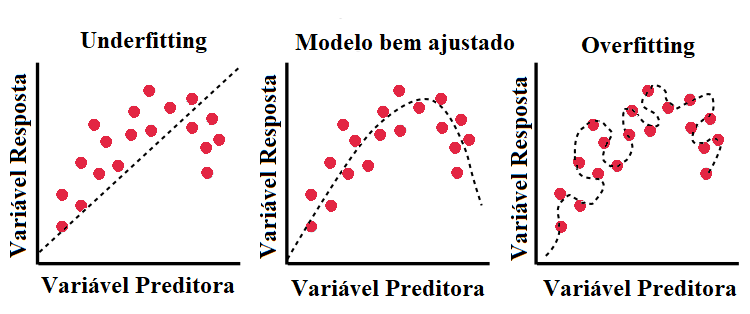
\includegraphics[width=0.7\linewidth]{G:/Hiro/Documents/Meus feitos/Livro ML/bookdown-demo-master/Figuras/graficofit} 

}

\caption{``Gráfico representando um \emph{Underfitting}, um Modelo bem ajustado e um \emph{Overfitting} respectivamente.''}\label{fig:graficofit}
\end{figure}



\hypertarget{validauxe7uxe3o-cruzada}{%
\section{Validação Cruzada}\label{validauxe7uxe3o-cruzada}}

A fim de que não haja previsões desastrosas geradas pelo modelo, para medirmos o desempenho real do modelo criado, é necessário que realizemos testes com ele, utilizando dados diferentes dos que foram apresentados no início. Portanto uma das técnicas mais utilizadas é a \textbf{Cross-validation (Validação Cruzada)}.

Após a realização do pré-processamento (analisar), iremos separar a totalidade dos dados históricos existentes em dois grupos, sendo o primeiro responsável pelo aprendizado do modelo, e o segundo por realizar os testes.
Seguindo o mesmo exemplo de bons ou mau pagadores, usualmente separamos o conjunto de dados dos clientes em duas amostras. Uma com

\hypertarget{como-escolher-um-bom-modelo}{%
\section{Como escolher um bom modelo?}\label{como-escolher-um-bom-modelo}}

  \bibliography{book.bib,packages.bib}

\end{document}
